%% Document class
\documentclass[iop,revtex4,numberedappendix,appendixfloats]{emulateapj}

%% General packages
\usepackage{amsmath}
\usepackage{mathrsfs }
\usepackage{lscape}

%% Figure packages
\usepackage{grffile}
\usepackage{subfigure}

%% Referencing
\usepackage{hyperref}

%% Custom macros
\newcommand{\vect}[1]{\boldsymbol{#1}}
\newcommand*\diff{\mathop{}\!\mathrm{d}}
\newcommand*\Diff[1]{\mathop{}\!\mathrm{d^#1}}
\newcommand{\pdf}{\ensuremath{pdf}}
\newcommand{\pmodel}{\ensuremath{p_M}}
\newcommand{\MAP}{MAP}
\newcommand{\MAPs}{MAPs}
\newcommand{\RM}{{\sl RoadMapping}}
\makeatletter
\newcommand{\testlabel}[2]{%
 \protected@write \@auxout {}{\string \newlabel {#1}{{#2}{\thepage}{#2}{#1}{}} }%
 \hypertarget{#1}{#2}
}
\makeatother

\usepackage[usenames,dvipsnames]{xcolor}
\newcommand{\Wilma}[1]{\textcolor{Magenta}{#1}}
\newcommand{\HW}[1]{\textcolor{Green}{#1}}
\newcommand{\Jo}[1]{\textcolor{Cyan}{#1}}

%% Symbols
\definecolor{darkorange}{HTML}{FF7F00}
\definecolor{brightorange}{HTML}{FDBF6F}
\definecolor{darkgreen}{HTML}{33A02C}
\definecolor{brightgreen}{HTML}{B2DF8A}
\usepackage{tikz}
\newcommand{\tikzcircle}[2][black,fill=black]{\tikz[baseline=-0.5ex]\draw[#1] (0,0) circle (#2);}%
\newcommand{\tikzsquare}[2][black,fill=black]{\tikz[baseline=-0.5ex]\draw[#1] ([xshift=-2pt,yshift=-2pt]10,0) rectangle ++(#2,#2);}%


%% Abbreviations
\shorttitle{Action-based Dynamical Modelling: The Influence of Spiral Arms}
\shortauthors{Trick et al.}

\begin{document}

%-----------------------------------------------------------------------------------------------------------------------------------------------------------------------------
%TITLE
%-----------------------------------------------------------------------------------------------------------------------------------------------------------------------------
\title{Action-based Dynamical Modelling for the Milky Way Disk:\\The Influence of Spiral Arms\\}

%% Authors
\author{Wilma H. Trick\altaffilmark{1,2}, Jo Bovy\altaffilmark{3}, Elena D'Onghia\altaffilmark{4,5}, and Hans-Walter Rix\altaffilmark{1}}

%% Affiliations
\altaffiltext{1}{Max-Planck-Institut f\"ur Astronomie, K\"onigstuhl 17, D-69117 Heidelberg, Germany}
\altaffiltext{2}{Correspondence should be addressed to trick@mpia.de.}
\altaffiltext{3}{Department of Astronomy and Astrophysics, University of Toronto, 50 St. George Street, Toronto, ON, M5S 3H4, Canada}
\altaffiltext{4}{Department  of  Astronomy,  University  of  Wisconsin,  2535 Sterling Hall, 475 N. Charter Street, Madison, WI 53076, USA}
\altaffiltext{5}{Alfred P. Sloan Fellow}

%-----------------------------------------------------------------------------------------------------------------------------------------------------------------------------
%ABSTRACT
%-----------------------------------------------------------------------------------------------------------------------------------------------------------------------------

\begin{abstract}
\RM{} is a well-tested dynamical modelling machinery developed to constrain the Milky Way's (MW) gravitational potential by simultaneously fitting an axisymmetric parametrized potential model and an axisymmetric action-based orbit distribution function (DF) to discrete 6D phase-space measurements of stars in the Galactic disk. In this work we demonstrate \RM{}'s robustness in the presence of spiral arms by modelling data drawn from a N-body simulation snapshot of a MW-like spiral galaxy in different survey volumes with radii $500~\text{pc} \leq r_\text{max} \leq 5~\text{kpc}$. The potential constraints are surprisingly successful \Jo{[TO DO: Jo writes: "Remove surprising, maybe robust."]}, even when using the most simple action-based DF, the quasi-isothermal DF (qDF). The best-fit \RM{} model always recovers the correct gravitational forces where most of the stars that entered the analysis are located. For data from large survey volumes \RM{} finds axisymmetric models that average well over the spiral arms. As expected, the models are slightly biased by the excess of stars in the spiral arms. Survey volumes with $r_\text{max}\leq 3~\text{kpc}$ give predictions for an overall axisymmetric potential as good as those from larger volumes. However, only for $r_\text{max}=5~\text{kpc}$ could the correct halo scale length be recovered. Potential models derived from small survey volumes ($r_\text{max} < 2~\text{kpc}$) centered on inter-arm regions can be more reliably used for extrapolation than those from small volumes affected by spiral arms. We discuss two possible applications of \RM{} to the stellar phase-space measurements from the upcoming Gaia data releases: (i) finding an overall axisymmetric potential model for the MW from data covering a large volume, (ii) measuring non-axisymmetric structures in the MW's disk by modelling data in small volumes independently. \Jo{[TO DO: Jo writes: "Need some sort of conclusion for these two."]} \Wilma{[TO DO: Currently 257 words. Might have to cut a few more.]}
\end{abstract}

%-----------------------------------------------------------------------------------------------------------------------------------------------------------------------------
%KEYWORDS
%-----------------------------------------------------------------------------------------------------------------------------------------------------------------------------
\keywords{Galaxy: disk --- Galaxy: fundamental parameters --- Galaxy: kinematics and dynamics --- Galaxy: structure --- \Wilma{[TO DO]}}

%-----------------------------------------------------------------------------------------------------------------------------------------------------------------------------
%INTRODUCTION
%-----------------------------------------------------------------------------------------------------------------------------------------------------------------------------
\section{Introduction}

The first step in learning more about the Milky Way's (MW) overall gravitational potential and orbit distribution function (DF)---which are crucial for understanding galaxy structure and formation \citep{013A&ARv..21...61R}---is to find the ``best possible'' axisymmetric model for the Galaxy. Given such a model the identification and characterization of non-axiysmmetries like the bar, spiral arms or stellar streams in stellar phase-space (and chemical abundance) data would then become more straightforward.

Several approaches to constrain an axisymmetric potential and/or orbit DF have recently been put forward: \citet{2013ApJ...779..115B} and \citet{2014MNRAS.445.3133P} fitted potential and DF simultaneously to stellar kinematics in the disk and got precise constraints on the overall potential; \citet{2015MNRAS.449.3479S} and \citet{2016MNRAS.460.1725D} investigated extended DFs for the disk and halo respectively (given a fiducial potential), that included in addition to the distribution in orbit space also the metallicity of each star. 

In this work we will continue our investigation of the \RM{} approach (\emph{``Recovery of the Orbit Action Distribution of Mono-Abundance Populations and Potential INference for our Galaxy''}). The first application of \RM{} was done by \citet{2013ApJ...779..115B} and \citet{2016arXiv160508601T}, hereafter Paper I, performed a detailed analysis of the strengths and weaknesses of the approach. The idea behind \RM{} is, that simple stellar populations in the MW disk---be it mono-abundance populations \citep{2012ApJ...751..131B,2012ApJ...753..148B,2012ApJ...755..115B,2016ApJ...823...30B} (i.e., stars with the same $[\mathrm{Fe}/\mathrm{H}]$ and $[\alpha/\mathrm{Fe}]$) or maybe also mono-age populations \citep{2013ApJ...773...43B,2014MNRAS.442.2474M,2016MNRAS.456.3655M,2014A&A...572A..92M,2016ApJ...823..114N}---follow simple orbit DFs, like, e.g., the quasi-isothermal DF (qDF) by \citet{2011MNRAS.413.1889B} \citep{2013MNRAS.434..652T}. The qDF is expressed in terms of the orbital actions $\vect{J}=(J_R,J_\phi=L_z,J_z)$, which are integrals of motion, quantify the amount of the orbit's oscillation in each of the coordinate directions $(R,\phi,z)$ and are therefore excellent orbit labels. Given an assumed gravitational potential one can calculate the orbital actions from the stars' current phase-space positions $(\vect{x},\vect{v})$ \citep{2012MNRAS.426.1324B,2016MNRAS.457.2107S} \Jo{[TO DO: Jo writes: "Bovy (2014) presents general method $(\vect{x},\vect{v})\longrightarrow(\vect{J},\vect{\theta})$."]}. Only if the assumed gravitational potential is realistic, this stellar action distribution will follow a realistic orbit DF like the qDF \Jo{[TO DO: Jo thinks the last half sentence is not very clear.]}. This allows one to simultaneously fit potential and orbit DF to observations.

\citet{2013ApJ...779..115B} employed this approach to measure the Milky Way's surface density profile within $1.1~\text{kpc}$ using 43 MAPs in the Galactic disk from the SDSS/SEGUE survey \citep{2009AJ....137.4377Y}. Their potential model had only two free parameters (disk scale length and relative halo-to-disk contribution to the radial force at the solar radius). To account for missing model flexibility they constrained the surface density for each MAP only at one best radius. The profile they derived in this fashion had a scale length of $R_s=2.5~\text{kpc}$ and was---in the regime $R>6.6~\text{kpc}$---later confirmed by \citet{2014MNRAS.445.3133P} using a different action-based procedure.

Given the success of this first application and in anticipation of the upcoming data releases from Gaia in 2016-2022 \citep{2013CEAB...37..115E}, Paper I improved the \RM{} machinery and studied its strengths and breakdowns in detail, by investigating a large suite of mock data sets. Under the prerequisite of axisymmetric data and model, they found that \RM{}'s modelling success is stable against minor misjudgements of DF or selection function, and that---if the true potential is not contained in the proposed family of model potentials---one can still find a good fit \Jo{[TO DO: Jo wants me to add "that returns the correct forces" here.]}, given the limitations of the model. Paper I also found that measurement uncertainties of the order of those by the final Gaia data release should be good enough (within $3~\text{kpc}$ from the Sun) to allow for precise and unbiased modelling results. 

The MW is, however, not axisymmetric. The bulge contains a strong bar \citep{1980ApJ...236..779L,1991ApJ...379..631B,2000MNRAS.317L..45H,2013MNRAS.435.1874W} and the disk itself is threaded by spiral arms \citep{1958MNRAS.118..379O,1976A&A....49...57G,2009PASP..121..213C,2014ApJ...783..130R} \Wilma{[TO DO: More references]} and (ring-like) overdensities \citep{2002ApJ...569..245N,2008ApJ...673..864J,2015ApJ...801..105X}, which induce non-circular motions and asymmetries in stellar number counts and correspond consequently to a non-axisymmetric gravitational potential and stellar DF. \Jo{[TO DO: Jo writes: "Could also cite kinematic evidence: moving groups (Eggen (????), \citet{1998AJ....115.2384D,2005A&A...430..165F,2009ApJ...700.1794B,2010ApJ...717..617B}) and streaming motions (in 21 cm or velocities) \citep{2015ApJ...800...83B,2013MNRAS.436..101W}, Siebert et al. 2013 or 2014)" $\longrightarrow$ Ich finde das Eggen und Siebert paper nicht ...]}

We are however planing to ultimately use an axisymmetric model to describe and model our non-axisymmetric Galaxy with \RM{}. This is an important breakdown of modelling assumptions which was not investigated in Paper I. But will \RM{} still be able to give reliable constraints on the MW's gravitational potential in the presence of spiral arms? Answering this question will be this work's objective.

Our investigation makes use of a N-body simulation snapshot of a spiral galaxy with strong spiral arms by \citet{2013ApJ...766...34D}. We draw mock data from this simulation in different regions with different spiral arm strengths and run the \RM{} machinery on these data sets and test how well we recover the local and overall gravitational potential.

In Paper I we tested and confirmed separately the robustness of \RM{} in the case that data came from a different model family of either potential or DF than assumed in the dynamical modelling. What would happen if both potential and DF model families were slightly wrong at the same time? The set-up of this study will automatically cover this important test case: The disk potential and orbit DF models that we are using are partly chosen because of their simplicity and computational advantages and---in case of the qDF---because that's what we are planning to use in the MW. We did not have any indications that they might be especially well-suited to describe an axisymmetric version of this simulated galaxy---quite the contrary.

A third modelling aspect that comes with the breakdown of axisymmetry in the data, is that the assumption actions being integrals of motion is not given anymore \citep{2016ApJ...824...39V} \Wilma{[TO DO: more references]}. This somewhat dilutes the advantages of using actions in the first place and it is not clear how well the orbit DF describes the distribution of instantaneous actions estimated in a slightly wrong and axisymmetric potential.

Overall, there are several reasons why the \RM{} modelling could result in severely biased potential constraints when applying it to the spiral galaxy simulation snapshot at hand---or directly to the MW, for that matter. Similar studies, like the ones by \citet{2013ApJ...779..115B,2014MNRAS.445.3133P,2015MNRAS.449.3479S} \Wilma{[TO DO: more references]}, implicitly assumed that the effect of the spiral arms should not matter too much. In this study we explicitely demonstrate that the \RM{} potential estimates are still surprisingly accurate, which makes us optimistic that they will be for the MW as well and were already in previous similar action-based modelling attempts.

This paper is organized as follows. Section \ref{sec:simulation} describes the N-body simulation snapshot of a MW-like spiral galaxy, that we are going to model in this study, explains how we extract 6D stellar phase-space data from it, and how we quantify the spiral arm strength. Section \ref{sec:RoadMapping} summarizes the \RM{} dynamical modelling framework and introduces the DF and potential model that will fit to the data. Section \ref{sec:results} is dedicated to presenting the results: In Section \ref{sec:results_part1} we discuss in detail the \RM{} modelling results derived from a data set within a survey volume with radius $r_\text{max}=4~\text{kpc}$ around the Sun. Section \ref{sec:results_part2} investigates then a whole suite of \RM{} analyses, corresponding to survey volumes of different sizes and different positions within the galaxy and with respect to the spiral arms. In Section \ref{sec:discussion} we discuss the results and conclude in Section \ref{sec:conclusion}.


%-----------------------------------------------------------------------------------------------------------------------------------------------------------------------------
%SIMULATION
%-----------------------------------------------------------------------------------------------------------------------------------------------------------------------------
\section{Data from a galaxy simulation} \label{sec:simulation}

%====================
\begin{figure}[!htbp]
\plotone{fig/plot_simulation_for_paper.pdf}
\caption{Simulation snapshot by \citet{2013ApJ...766...34D} . Shown are the surface mass density (in $(x,y)$ plane, upper panel) and mass density (in $(R,z)$ plane, lower panel) of the ``star'' particles belonging to disk, bulge and giant molecular clouds. (The dark matter halo in this simulation is static and analytic and not shown here.) Overplotted are the disk's scale length $R_s=2.5~\text{kpc}$ (see Section \ref{sec:simulation_description}) and the radii at which we center our test survey volumes in this investigation, $R=8$ and $5~\text{kpc}$. The centers of the different survey volumes are marked with a square, if the survey volume is centered on a spiral arm, or with a circle, if the volume is centerd on an inter-arm region. The yellow circle with radius $r_\text{max}=4~\text{kpc}$ marks the survey volume in which we conduct the analysis discussed in detail in Section \ref{sec:results_part1}. \Wilma{[TO DO: overplot names of positions.]}}
\label{fig:simulation}
\end{figure}
%====================

\subsection{Description of the galaxy simulation snapshot} \label{sec:simulation_description}

In this work we use stellar phase-space data drawn from high-resolution N-body simulation snapshot of a disk galaxy by \citet{2013ApJ...766...34D} carried out with GADGET-3 code described in \citet{2005MNRAS.361..776S}, in which overdensities with properties similar to giant molecular clouds induced prominent spiral arms---and therefore non-axisymmetric sub-structure---via the swing amplification mechanism. 

For details see \citet{2013ApJ...766...34D}, here we summarize the essential characteristics.

The simulation has a gravitationally evolving stellar disk within a static/rigid analytic dark matter halo.

The analytic halo follows a \citet{1990ApJ...356..359H} profile
\begin{equation}
\rho_\text{dm}(r) = \frac{M_\text{dm}}{2\pi} \frac{a_\text{dm}}{r (r+a_\text{dm})^3} \label{eq:dm_hernquist}
\end{equation}
with total halo mass $M_\text{dm} = 9.5\cdot 10^{11} ~M_\odot$ and scale length $a_\text{dm} = 29~\text{kpc}$ (Elena D'Onghia, private communication).

The disk consists of $10^8$ ``disk star'' particles, each having a mass of $\sim370 ~M_\odot$, and 1000 ``giant molecular cloud'' particles with mass $\sim9.5\cdot 10^{5} ~M_\odot$. Initially the particles are distributed following an exponential disk profile with density
\begin{equation}
\rho_*(R,z) = \frac{M_*}{4\pi z_0 R_s^2} \text{sech}^2 \left( \frac{z}{z_0}\right) \exp \left(- \frac{R}{R_s} \right), \label{eq:sech_disk}
\end{equation}
with $R_s = 2.5~\text{kpc}$ and $z_0=0.1R_s$ and total disk mass $M_* = 0.04\cdot M_\text{dm} = 3.8\cdot 10^{10} M_\odot$ .

The bulge consists of $10^7$ ``bulge star'' particles with mass $\sim950 ~M_\odot$ and they are distributed following a spherical Hernquist profile analogous to Equation \eqref{eq:dm_hernquist}, with total mass $M_\text{bulge}=0.01 \cdot M_\text{dm} = 9.5\cdot 10^9~M_\odot$ and scale length $a_\text{bulge}=0.1\cdot R_s=0.25~\text{kpc}$.

The simulation snapshot which we are using in this work has evolved under its own gravity for $\sim 250~\text{Myr}$, which corresponds to approximately one orbital period at $R\sim8~\text{kpc}$. The mass density of simulation particles (without the DM halo) at this snapshot time is shown in Figure \ref{fig:simulation}. Pronounced spiral arms have developed due to the ``molecular cloud perturbers'', which can be seen in Figure \ref{fig:simulation} as small overdensities in the disk. The spherical bulge and very flattened disk are shown in the lower panel in Figure \ref{fig:simulation}.

We have confirmed that the gravitational center of the particles corresponds to the coordinate origin.

\subsection{Survey volume and data}

%====================
\begin{deluxetable}{clccc}[!htbp]
\tabletypesize{\scriptsize}
\tablecaption{Vantage points within the galaxy simulation snapshot around which we center survey volumes of radius $r_\text{max}$. \label{tbl:volume_positions}}
\tablewidth{0pt}
\tablehead{
\colhead{name} & \colhead{position} & \colhead{$R_0$ [kpc]} & \colhead{$\phi_0$ [degrees]} & \colhead{legend}}
\startdata
\tableline
\texttt{S8} & on spiral arm & 8 & 5 & \tikzsquare[fill=darkorange]{6pt}\\
\texttt{I8} & in inter-arm region & 8 & -15 &  \tikzcircle[fill=brightorange]{3pt}\\
\texttt{S5} & on spiral arm & 5 &  60 & \tikzsquare[fill=darkgreen]{6pt}\\
\texttt{I5} & in inter-arm region & 5 & 0 & \tikzcircle[fill=brightgreen]{3pt}
\enddata
\tablecomments{All volumes are centered on $z_0=0$ in the plane of the disk, and $\phi_0$ is measured counter-clockwise from the positive $x$-coordinate axis.}
\end{deluxetable}

The selection function of all-sky surveys like Gaia, that are only limited by the brightness of the tracers, are contiguous and---when ignoring anisotropic effects like dust obscuration---spherical in shape. For simplicity we will use spherical survey volumes centered on different vantage points and with sharp edges at a radius $r_\text{max}$ around it (see also Section \ref{sec:likelihood}), which corresponds to a magnitude cut for stellar tracers all having the same luminosity. 

Figure \ref{fig:simulation} illustrates the different survey volume positions we use in this study: We use each a volume with $r_\text{max}=1,2,3,4$ or $5~\text{kpc}$ centered on a spiral arm and on an inter-arm region at both the equivalent of the solar radius in this simulation, $R=8~\text{kpc}$, and at $R=5~\text{kpc}$, where the spiral arms are more pronounced (see Figure \ref{fig:spiral_arm_kappa}) than at $R=8~\text{kpc}$. The exact positions of the vantage points are summarized in Table \ref{tbl:volume_positions}.

From each volume we draw $N_*=20,000$ random ``disk star'' particles from the simulation and use their phase-space positions $(\vect{x}_i,\vect{v}_i)$ within the simulated galaxy's restframe as data. 

To make the data sample more realistic, one would actually have to add measurement uncertainties, especially to the distances from the survey volume's central vantage point and the proper motions measured from there. We decided not to include measurement uncertainties: Firstly, their effect on \RM{} modelling has been already investigated in Paper I and we found that the measurement uncertainties of the last data release of Gaia should be small enough to not disturb the modelling to much. Secondly, in this study we want to isolate and investigate the deviations of the data from the assumed potential and DF model and axisymmetry independently of other effects.

\subsection{Symmetrized potential model} \label{sec:DEHH-Pot}

For a galaxy with pronounced spiral arms an axisymmetric model matter distribution can per se not reproduce the true matter distribution globally. We derived an \emph{overall best fit symmetrized} potential model from the distribution of particles to be able (i) to quantify the non-axisymmetries in the simulation snapshot better and (ii) to compare how close our axisymmetric \RM{} results can get to it. 

We derive this model by fitting axisymmetric analytical functions to the density distribution of each of the galaxy component's particles: The bulge and halo follow each a Hernquist profile by construction (see Section \ref{sec:simulation_description}). The disk with its spiral arms however does deviate strongly from its initial conditions in Equation \ref{eq:sech_disk}. We chose a double exponential disk model to fit the particle distribution in the disk. The best fit parameters for this reference potential, to which we will refer as the \texttt{DEHH-Potential} (Double-Exponential disk + Hernquist halo + Hernquist bulge) in the remainder of this work, are given in Table \ref{tbl:DEHH-Pot}. As can be seen in Figures \ref{fig:4kpc8Spiral_density} and \ref{fig:4kpc8Spiral_vcirc_surfdens} in Section \ref{sec:results_part1} below, the \texttt{DEHH-Pot} fits the overall density distribution very well. Its density profile might be a little stepper around $z\sim 0$ than the actual particle distribution, but this should not affect the overall discussion, as the radial density, surface density and disk-to-halo ratio profiles are so well reproduced.

%Reference for sech(z) disk: http://adsabs.harvard.edu/abs/1989MNRAS.239..571K If I really need to evaluate it...

%====================
\begin{deluxetable}{lll}[!htbp]
\tabletypesize{\scriptsize}
\tablecaption{Best fit parameters of the \texttt{DEHH-Pot} (see Section \ref{sec:DEHH-Pot}), which we use as the global best fit symmetrized potential model. \label{tbl:DEHH-Pot}}
\tablewidth{0pt}
\startdata
\tableline
circular velocity & $v_\text{circ}(R_\odot)$ & $222~\text{km s}^{-1}$ \\
disk scale length & $h_r$ & $2.5~\text{kpc}$ \\
disk scale height & $h_z$ & $0.17~\text{kpc}$ \\
halo fraction & $f_\text{halo}$ & $0.54$\\
halo scale length & $a_\text{halo}$ & $29~\text{kpc}$ \\
bulge mass & $M_\text{bulge}$ & $0.95 \cdot 10^{10}M_\odot$\\
bulge scale length & $a_\text{bulge}$ & $0.25~\text{kpc}$
\enddata
%\tablenotetext{(a)}{...}
\tablecomments{The halo fraction, $f_\text{halo}$, and circular velocity at the Sun, $v_\text{circ}(R_\odot)$, which scales the total mass of the model, are defined in Equations \eqref{eq:fhalo} and \eqref{eq:circvel}.}
\end{deluxetable}
%====================

\subsection{Quantifying influence of spiral arm} \label{sec:spiral_arm_kappa}

Depending on size and position of the survey volume the spiral arms and inter-arm regions dominate the stellar distribution within the survey volume to different degrees. To quantify the strength of the spiral arm, we introduce the quantity
\begin{equation}
\kappa(x_j,y_j) \equiv \frac{\Sigma_{\text{disk},T}(x_j,y_j \mid |z|\leq 1.5~\text{kpc})}{\Sigma_{\text{disk},S}(x_j,y_j \mid |z| \leq1.5~\text{kpc})} -1\label{eq:kappa_definition}
\end{equation}
where $\Sigma_{\text{disk},i}$ is the surface density of the disk component  of the simulation snapshot ($i=T$) or of the symmetrized snapshot model \texttt{DEHH-Pot} in Section \ref{sec:DEHH-Pot} ($i=S$) within the survey volume,
\begin{equation}
\Sigma_{\text{disk},i} \equiv \int_{-1.5~\text{kpc}}^{1.5~\text{kpc}} \rho_{\text{disk},i}(x_j,y_j,z) \ \diff z.
\end{equation}
$(x_j,y_j)$ is the centroid of a surface area element $(x_j\pm\delta,y_j\pm \delta)$ with $\delta=0.25~\text{kpc}$. $(x_c=R_{0,c}\times\cos \phi_{0,c},y_c=R_{0,c}\times\sin \phi_{0,c},z_c=0)$ is the position of the survey volume's center within the simulation, with $c\in\left\{ \texttt{S8},\texttt{I8},\texttt{S5},\texttt{I5}\right\}$ and $(R_{c,0},\phi_{c,0})$ given in Table \ref{tbl:volume_positions}. We consider all $n \simeq \pi r_\text{max}^2/4\delta^2$ values of $\kappa(x_j,y_j)$ inside a given survey volume of radius $r_\text{max}$ around position $c$ and calculate the mean and standard deviation,
\begin{eqnarray}
\langle \kappa \rangle \equiv \langle \kappa (r \leq r_\text{max} \mid c) \rangle &\equiv & \frac 1n \sum_{j=1}^n \kappa(x_j,y_j)\label{eq:mean_kappa}\\
\sigma_\kappa \equiv \sigma[\kappa(r \leq r_\text{max} \mid c)]  &\equiv &  \sqrt{\frac 1n \sum_{j=1}{n} \left[ \kappa(x_j,y_j) -  \langle \kappa \rangle \right]^2}\label{eq:std_kappa}\\
 \text{with } && (x_j-x_c)^2 + (y_j-y_c)^2 \leq r_\text{max}. \nonumber
\end{eqnarray}
This gives us information if a spiral arm or an inter-arm region dominates the survey volume ($\langle \kappa \rangle > 0$ for spiral arms, $\langle \kappa \rangle < 0$ for inter-arm regions) and how large the relative contrast between spiral arms and inter-arm regions is ($\sigma_\kappa$). For example, small volumes sitting completely within an inter-arm region, or large volumes that contain---in addition to some spiral arms and depleted inter-arm regions---also large areas of unperturbed disk, will have an overall small relative spiral contrast $\sigma_\kappa$.

%====================
\begin{figure*}[!htbp]
\centering
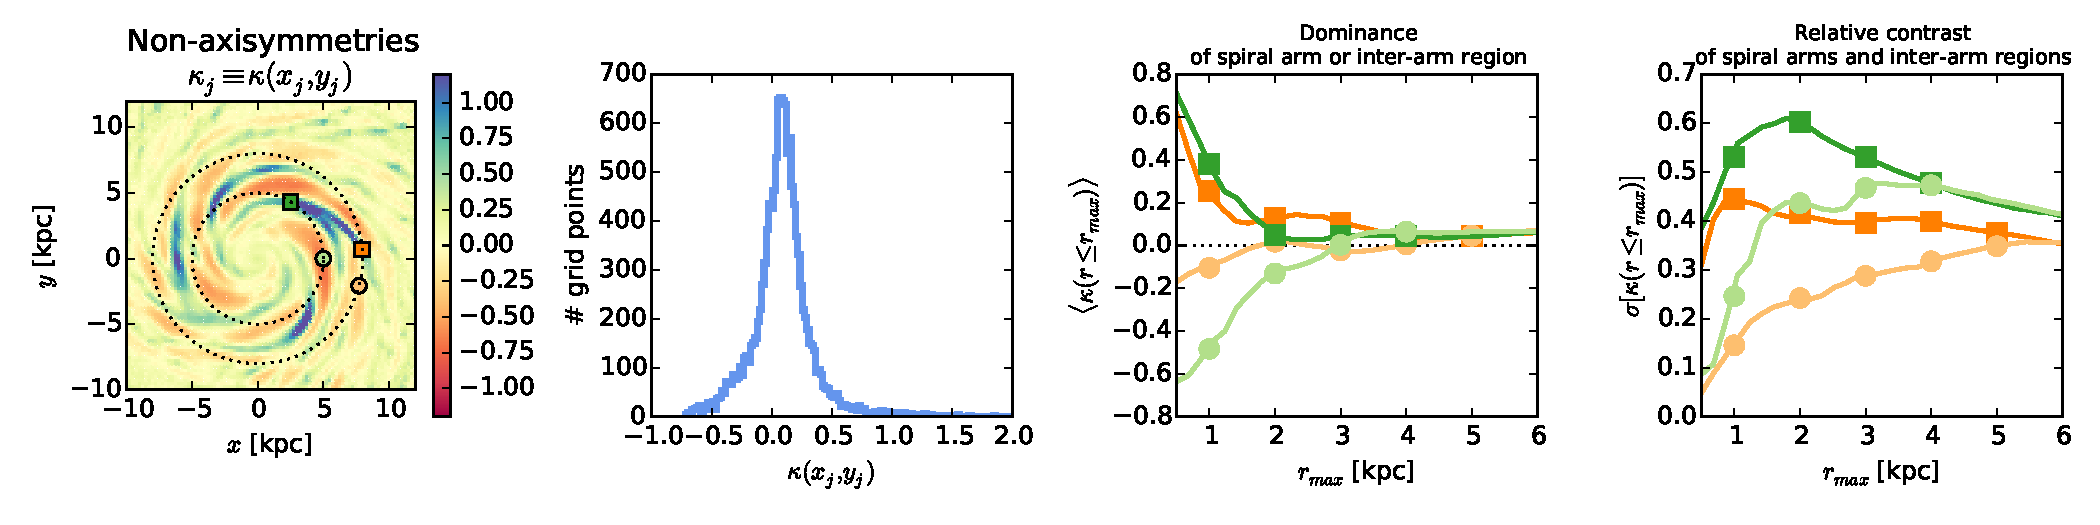
\includegraphics[width=\textwidth]{fig/whole_galaxy_kappa_i.pdf}
\caption{Contrast and dominance of the spiral arms. The left panel shows the values of $\kappa_i$ calculated according to Equation \ref{eq:kappa_definition} as described in Section \ref{sec:spiral_arm_kappa} at regular grid points $(x_i,y_i)$ with bin width $0.25~\text{kpc}$. Marked are the centroids of the four test survey volumes of this study. The second panel shows a histogram over all $kappa(x_j,y_j)$ values in the region $x,y \in [-14,14]~\text{kpc}$. The two right panels show the dominance (with the mean $\langle \kappa (r \leq r_\text{max} \rangle$ of all grid points within the survey volume as measure) and the relative contrast (with the standard deviation $\sigma[\kappa (r \leq r_\text{max})]$ as measure) of spiral arms and inter-arm regions inside a spherical survey volume with given centroid (colour-coded) and size (radius $r_\text{max}$ shown on the $x$-axis). We chose two volumes in which the spiral arms dominate, and two in which an inter-arm region dominates. The dominance and contrast of spiral arms and inter-arm regions is stronger at $R=5~\text{kpc}$ than at $R=8~\text{kpc}$. Also, inter-arm regions appear larger and smoother than spiral arms, as already inside a small volume centred on a spiral arm the contrast is quite large. The larger the volume the more does the overall effect of spiral arms and inter-arm regions average out. \Wilma{[TO DO: Add dots for the $r_\text{max}=500~\text{kpc}$ volumes.]} \HW{[TO DO: Jo suggested to look into implementing a $\text{sech}^2$ disk for galpy to not have the slight bias in mean($\kappa$) at higher rmax. Maybe it's easy to implement. Maybe it isn't.]}}
\label{fig:spiral_arm_kappa}
\end{figure*}
%====================


%-----------------------------------------------------------------------------------------------------------------------------------------------------------------------------
%MODELLING
%-----------------------------------------------------------------------------------------------------------------------------------------------------------------------------
\section{RoadMapping modelling} \label{sec:RoadMapping}

\subsection{Likelihood} \label{sec:likelihood}

The data that goes into the modelling are the 6D position and velocity coordinates $(\vect{x}_i,\vect{v}_i)$ of $N_*$ stars within the survey volume. For simplicity we use a purely spatial selection function $\text{sf}(\vect{x})$ of spherical shape,
\begin{equation*}
\text{sf}(\vect{x}) \equiv \begin{cases} 1 &\mbox{if } \left| \vect{x}-\vect{x}_0 \right| \leq r_\text{max} \\
0 & \mbox{otherwise} \end{cases},
\end{equation*}
whose maximum radius $r_\text{max}$ defines the boundary of the survey volume and which is centred on $\vect{x}_0 \equiv (R_0,\phi_0,z_0=0)$. Given a parametrized potential model $\Phi(R,z)$ with parameters $p_\Phi$, the $i$-th star is on an orbit characterized by the orbital actions 
\begin{equation*}
\vect{J}_i \equiv \vect{J}[\vect{x}_i,\vect{v}_i \mid p_\Phi].
\end{equation*}
The probability of stars to be on the orbit $\vect{J}_i$ is proportional to a given orbit distribution function $\text{df}(\vect{J})$ with parameters $p_\text{DF}$,
\begin{equation*}
\text{df}(\vect{J}_i \mid p_\text{DF}) \equiv \text{df}(\vect{J}[\vect{x}_i,\vect{v}_i \mid p_\Phi] \mid p_\text{DF}) \equiv \text{df}(\vect{x}_i,\vect{v}_i \mid p_\Phi,p_\text{DF}),
\end{equation*} 
where the latter equivalence arises from the Jacobian determinant between the angle-action coordinates $(\vect{\theta},\vect{J})$ and cartesian phase-space coordinates $(\vect{x},\vect{v})$, which is $\left| \partial (\vect{x},\vect{v}) / \partial(\vect{\theta},\vect{J})\right|=1$ and therefore allows us to treat the $\text{df}$ equivalently as a distribution of current phase-space coordinates or a distribution of orbital actions only, with uniform distribution in the angles $\vect{\theta}$. In some sense, the $\text{df}(\vect{J})$ describes how we expect a realistic stellar population in the MW disk to look like.

The joint likelihood of the $i$-th star being on an orbit $\vect{J}$ in the potential $\Phi$ and being within the survey volume is therefore
\begin{equation*}
\mathscr{L}_i \equiv \mathscr{L}(\vect{x}_i,\vect{v}_i) = \frac{\text{df}(\vect{x}_i,\vect{v}_i\mid p_\phi, p_\text{DF}) \cdot \text{sf}(\vect{x_i})}{\int \text{df}(\vect{x},\vect{v}\mid p_\Phi, p_\text{DF}) \cdot \text{sf}(\vect{x}) \ \Diff3 x \Diff3 v}.
\end{equation*}
The details how we evaluate the likelihood normalisation numerically to sufficiently high enough precision are discussed in Paper I.\footnote{In the terminology of Paper I we use the high numerical accuracy $N_x = 20$, $N_v = 28$, $n_\sigma = 5.5$ to calculate the likelihood normalisation, or in other words, to evaluate the spatial and velocity integrals over the qDF within the survey volume. For the action interpolation grid following \citet{2015ApJS..216...29B}, we use $R_\text{max}=40~\text{kpc}$, $n_E=70$, $n_\psi=40$, $n_{L_z}=50$ in their terminology.}

In the scenario considered in this paper it can happen that there are a few ($\sim 1$ in 20,000) stars entering the catalogue that are for some reason  on rather extreme orbits, e.g., moving radially directly towards the center. These kinds of orbits do not belong to the set of orbits that we classically expect to make up a overall smooth galactic disk. To avoid that such single stars with very low likelihood mess up the modelling we introduce here a simple outlier model,
\begin{equation*}
\mathscr{L}_i \longrightarrow \max \left( \mathscr{L}_i, \epsilon \cdot \text{median}(\mathscr{L})\right),
\end{equation*}
where $\epsilon = 0.001$ for $N_*=20,000$ stars and $\text{median}(\mathscr{L})$ is the median of all the $N_*$ stellar likelihoods $\mathscr{L}_i$ with the given $p_\Phi$ and $p_\text{DF}$. This outlier model was not used in Paper I.

Following Paper I, we assume for now uninformative flat priors on the model parameters $p_\Phi$ and $p_\text{DF}$ and find the maximum and width of the posterior probability function
\begin{equation*}
pdf(p_\Phi,p_\text{DF} \mid \text{data}) \propto \prod_{i=1}^{N_*} \mathscr{L}_i \cdot prior(p_\Phi,p_\text{DF})
\end{equation*}
using a nested-grid approach and then explore the full shape of the $\pdf$ using a Monte Carlo Markov Chain (MCMC)\footnote{We use the MCMC software \emph{emcee: The MCMC Hammer} by \citet{2013PASP..125..306F}.}. Full details on this procedure are given in Paper I.

\subsection{DF model} \label{sec:DF_model}

The most simple orbit distribution function exhibiting a disk-like structure may be the quasi-isothermal distribution function (qDF) introduced by \citet{2010MNRAS.401.2318B} and \citet{2011MNRAS.413.1889B}. It  proofed to be a successful model to describe the orbit distribution of individual mono-abundance populations (MAPs) in the Galactic disk \citep{2013ApJ...779..115B,2013MNRAS.434..652T}, that seem to be isothermal in $z$-direction (i.e., ``quasi-isothermal''). Modelling approaches trying to capture the overall disk distribution \citep{2014MNRAS.445.3133P,2015MNRAS.449.3479S} were describing the Galactic disk as a superposition of many qDFs. The qDF, which we already used in Paper I, has the functional form
\begin{eqnarray}
&&\text{qDF}(\vect{J} \mid p_\text{DF}) \nonumber\\
&&= f_{\sigma_R}\left(J_R,L_z \mid p_\text{DF}\right) \times f_{\sigma_z}\left(J_z,L_z \mid p_\text{DF}\right)\label{eq:df_general}\end{eqnarray}
where
\begin{eqnarray}
f_{\sigma_R}\left(J_R,L_z \mid p_\text{DF}\right) &=& n \times \frac{\Omega}{\pi\sigma_R^2(R_g) \kappa}\exp\left(-\frac{\kappa J_R}{\sigma_R^2(R_g)} \right) \nonumber\\
&& \times \left[1+\tanh\left(L_z/L_0\right) \right]\\
f_{\sigma_z}\left(J_z,L_z \mid p_\text{DF} \right) &=& \frac{\nu}{2 \pi \sigma_z^2(R_g)} \exp\left( -\frac{\nu J_z}{\sigma_z^2(R_g)} \right)
\end{eqnarray}
\citep{2011MNRAS.413.1889B}. The guiding-center radius $R_g$, circular frequency $\Omega$, radial/epicycle frequency $\kappa$ and vertical frequency $\nu$ describe the near-circular orbit with given angular momentum $L_z$ in a given potential. Counter-rotating orbits with $L_z < L_0$ are suppressed by the term $\left[1+\tanh\left(L_z/L_0\right) \right]$ (with $L_0 \sim 10~\text{km s}^{-1}~ \text{kpc}$). 
We set the radial stellar tracer density $n(R_g)$ and velocity dispersion profiles $\sigma_z(R_g)$ and $\sigma_R(R_g)$ to
\begin{eqnarray}
n(R_g \mid p_\text{DF}) &\propto& \exp\left(-\frac{R_g}{h_R} \right)\\
\sigma_R(R_g \mid p_\text{DF}) &=& \sigma_{R,0} \times \exp\left(- \frac{R_g-R_\odot}{h_{\sigma,R}} \right)\label{eq:sigmaRRg}\\
\sigma_z(R_g \mid p_\text{DF}) &=& \sigma_{z,0} \times \exp\left(- \frac{R_g-R_\odot}{h_{\sigma,z}} \right)\label{eq:sigmazRg}.
\end{eqnarray}
The free model parameters of the qDF are therefore
\begin{equation*}
p_\text{DF} \equiv \left\{ \ln h_R, \ln \sigma_{R,0}, \ln \sigma_{z,0}, h_{\sigma,R}, h_{\sigma,z}\right\}.
\end{equation*}

Even though we do not have any stellar abundance or age information in the simulation snapshot we are going to investigate (see Section \ref{sec:simulation_description}) and we therefore cannot define stellar sub-populations for which the assumption of such a simple model might be reasonable, we will still try to model the whole disk with a single qDF---to see how far we can get with the simplest possible model.

\subsection{Potential model} \label{sec:potential_model}

%====================
\begin{deluxetable*}{lll}[!htbp]
\tabletypesize{\scriptsize}
\tablecaption{Best-fit \texttt{MNHH-Pot} and qDF parameters as recovered from the \RM{} analysis of a survey volume with $r_\text{max}=4~\text{kpc}$ centered on a spiral arm at $R_0=8~\text{kpc}$ (position \texttt{S8}). \label{tbl:MNHHdiffSph2_4kpc8Spiral}}
\tablewidth{0pt}
\startdata
\tableline
circular velocity & $v_\text{circ}(R_\odot)$ & $(223.0 \pm 0.1) ~\text{km s}^{-1}$\\
Miyamoto-Nagai disk scale length & $a_\text{disk}$ & $(3.62^{+ 0.06}_{- 0.05}) ~\text{kpc}$\\
Miyamoto-Nagai disk scale height & $b_\text{disk}$ & $(0.26 \pm 0.02) ~\text{kpc}$\\
halo fraction & $f_\text{halo}$ & $(0.53 \pm 0.02)$\\
halo scale length & $a_\text{halo}$ & $(21 \pm 2) ~\text{kpc}$\\
bulge mass & $M_\text{bulge}$ & $0.95 \cdot 10^{10}M_\odot$ (fixed)\\
bulge scale length & $a_\text{bulge}$ & $0.25~\text{kpc}$ (fixed)\\
\tableline
qDF tracer scale length & $h_R$ & $3.34^{+ 0.05}_{- 0.04} ) ~\text{kpc}$\\
qDF radial velocity dispersion & $\sigma_{R,0}$ & $15.91 \pm 0.08) ~\text{km s}^{-1}$\\
qDF vertical velocity dispersion & $\sigma_{z,0}$ & $14.0^{+ 0.2}_{- 0.1}) ~\text{km s}^{-1}$\\
qDF radial velocity dispersion scale length & $h_{\sigma,R}$ & $(4.6 \pm 0.5)~\text{kpc}$\\
qDF vertical velocity dispersion scale length & $h_{\sigma,z}$ & $(5.65^{+ 0.06}_{- 0.07}) ~\text{kpc}$
\enddata
%\tablenotetext{(a)}{...}
\tablecomments{The bulge mass and scale length were fixed in the analysis to their true values, see Sections \ref{sec:simulation_description} and \ref{sec:potential_model}.}
\end{deluxetable*}
%====================

\Wilma{[TO DO: each equation should have a number]}

In all \RM{} analyses in this work we will fit an axisymmetric gravitational potential model to the data consisting of a (fixed and known) Hernquist bulge, a free Hernquist halo and a free Miyamoto-Nagai disk \citep{1975PASJ...27..533M},
\begin{equation}
\Phi_\text{disk}(R,z) = - \frac{GM}{\sqrt{R^2+(a_\text{disk}+\sqrt{z^2+b_\text{disk}^2})^2}}, \label{eq:MN-disk}
\end{equation}
where $a_\text{disk}$ and $b_\text{disk}$ are the equivalents of a disk scale length and scale height. To use Hernquist profiles for halo and bulge is motivated by our knowledge of the snapshot galaxy, and we fix the bulge's total mass and scale length to the true values (see Section \ref{sec:simulation_description} and Table \ref{tbl:MNHHdiffSph2_4kpc8Spiral}). As the bulge contribution to the total radial force at $R=8~\text{kpc}$ is only $\sim9-10\%$, this will not give the modelling an "unfair advantage". The free model parameters of the halo are the halo scale length $a_\text{halo}$ and the relative halo-to-disk contribution to the radial force, i.e.,
\begin{equation}
f_\text{halo} \equiv \frac{F_\text{R,halo}}{F_\text{R,disk} + F_\text{R,halo}}.\label{eq:fhalo}
\end{equation}
As parameter that scales the total mass of the galaxy model we use the circular velocity at the "solar" radius,
\begin{equation}
v_\text{circ}(R_\odot=8~\text{kpc}) \equiv \left. \sqrt{ R \frac{\partial \Phi}{\partial R} }\right|_{\stackrel{R=R_\odot}{z=0}} . \label{eq:circvel}
\end{equation}  
The total set of free potential model parameters is therefore
\begin{equation}
p_\Phi \equiv \left\{ v_\text{circ}(R_\odot),a_\text{disk},b_\text{disk},a_\text{halo},f_\text{halo}\right\}.
\end{equation} 
We will call this potential model the \texttt{MNHH-Pot} (Miyamoto-Nagai disk + Hernquist halo + Hernquist bulge) in the remainder of this work.

To estimate the stellar actions $\vect{J}=(J_R,L_z,J_z)$ in the axisymmetric \texttt{MNHH-Pot}, we are using the \emph{St\"{a}ckel fudge} algorithm by \citet{2012MNRAS.426.1324B}, which is the best compromise between speed and accuracy and especially well-suited for action estimations in a thin disk (see \citealt{2016MNRAS.457.2107S}). To speed up the code even more, we also interpolate the actions on a grid \citep{} and used a fixed St\"{a}ckel focal length of $\Delta=0.45$ for the \emph{St\"{a}ckel fudge}. We made sure, that the accuracy of the parameter estimates are not degraded by interpolation errors.

For the potential models and the qDF, as well as the  \emph{St\"{a}ckel fudge}, \RM{} makes extensive use of the \texttt{galpy} python library by \citet{2015ApJS..216...29B}\footnote{The \texttt{galpy} (galaxy python) package by \citet{2015ApJS..216...29B} can be downloaded from \url{http://github.com/jobovy/galpy}.}.

The \texttt{DEHH-Pot} introduced in Section \ref{sec:DEHH-Pot} with its double-exponential disk profile is better than the Miyamoto-Nagai disk in reproducing the overall radial density slope, as we will see in Figures \ref{fig:4kpc8Spiral_density} and \ref{fig:4kpc8Spiral_vcirc_surfdens} in the next section, and which is also suggested by the inital disk configuration in Equation \ref{eq:sech_disk}. However, the closed from expression of the potential in Equation \eqref{eq:MN-disk} has the crucial advantage of allowing very fast force and therefore action calculations in \RM{} modelling. And the gain in computational speed as compared to using the \texttt{DEHH-Pot}, which requires the evaluation of integrals and Bessel functions to calculate the forces, is essential. In addition, by using a potential model where we already know that it is not be the optimal model for the galaxy's disk, we challenge \RM{} even further.

How should one compare the \RM{} results for the best-fit \texttt{MNHH-Pot} with the fixed \texttt{DEHH-Pot} (Table \ref{tbl:DEHH-Pot}) in the remainder of this work? When considering \emph{a global} best fit potential model for the galaxy, \RM{} model can not be better than the \texttt{DEHH-Pot}, which is therefore a global upper limit for \RM{}'s modelling success. We note that in deriving the \texttt{DEHH-Pot} in Section \ref{sec:DEHH-Pot} we used the correct decomposition into bulge, disk and halo components. \RM{} however is only sensitive to the composite gravitational effect of the potential. Given the flexibility of the \texttt{MNHH-Pot} model used in \RM{} and the restriction of the modelling to a survey volume, it could be possible that \RM{} can do better in fitting the local potential inside the survey volume at the price of recovering the global potential parameters to less accuracy. We will discuss this in the following sections.

%-----------------------------------------------------------------------------------------------------------------------------------------------------------------------------
%RESULTS
%-----------------------------------------------------------------------------------------------------------------------------------------------------------------------------
\section{Results} \label{sec:results}

We run the \RM{} modelling on several data sets drawn from different survey volumes in the simulation snapshot introduced in Section \ref{sec:simulation_description}. In Section \ref{sec:results_part1} we will analyze one of these \RM{} analyses in detail, and in Section \ref{sec:results_part2} we compare the different results for the different data sets.

%====================
\begin{figure*}[!htbp]
  \centering
  \subfigure[DF density residuals.\label{fig:DF_densres}]{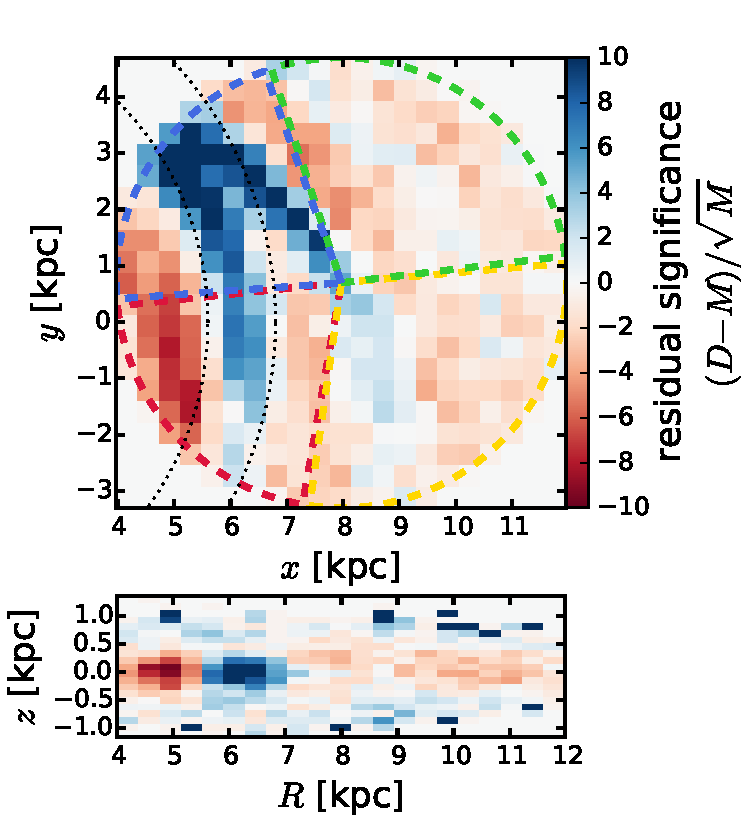
\includegraphics[width=0.32\linewidth]{fig/MNdHHdiffSph2_4kpc8Spiral_a_test1_data_bestfit_residuals_3a.pdf}}
  \subfigure[DF density profiles.\label{fig:DF_densprof}]{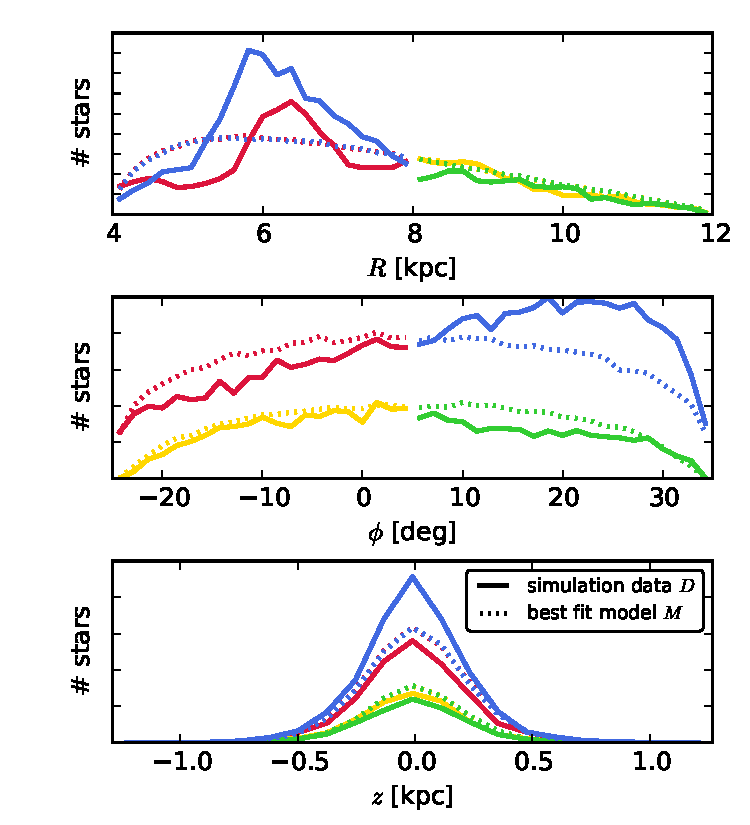
\includegraphics[width=0.32\linewidth]{fig/MNdHHdiffSph2_4kpc8Spiral_a_test1_data_bestfit_residuals_3b.pdf}}
  \subfigure[DF velocity residuals.\label{fig:DF_velres}]{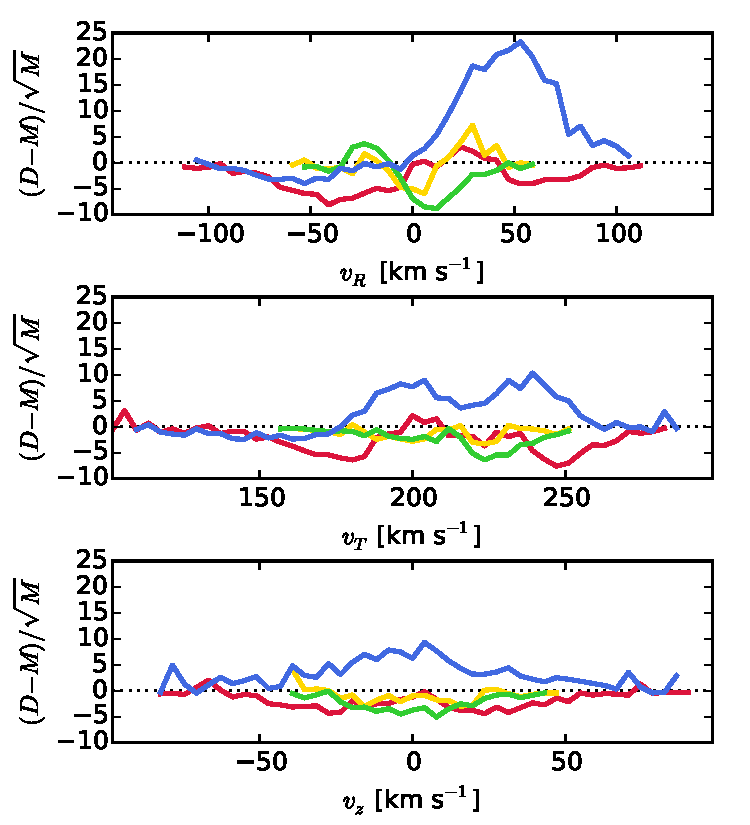
\includegraphics[width=0.32\linewidth]{fig/MNdHHdiffSph2_4kpc8Spiral_a_test1_data_bestfit_residuals_3c.pdf}}
  \caption{Comparison of the DF of stars in position-velocity space in the data set from the simulation snapshot (with $N_*=20,000$ and $r_\text{max}=4~\text{kpc}$ centered on position \texttt{S8}) and in the single-qDF best fit \RM{} model from Table \ref{tbl:MNHHdiffSph2_4kpc8Spiral}. Panel \ref{fig:DF_densres} shows the spatial density residual significance projected to the $(x,y)$ and $(R,z)$ plane. In the $(x,y)$ panel the following regions are marked: $R<8~\text{kpc},\phi>5^\circ$ (blue), $R<8~\text{kpc},\phi<5^\circ$ (red), $R>8~\text{kpc},\phi>5^\circ$ (green), $R>8~\text{kpc},\phi<5^\circ$ (yellow). Panels \ref{fig:DF_densprof} and \ref{fig:DF_velres} show the density profiles and velocity residual significance along each of the 6D phase-space coordinates separately for each of the four spatial regions. The blue region is very much dominated by the non-axisymmetric spiral arm. For the yellow region the axisymmetric single-qDF model is a good description. Overall the qDF is a good average axisymmetric model for the data. (In panel \ref{fig:DF_densres} we overplot the radii $R_\text{spiral} \in [5.6,6.8]~\text{kpc}$ as black dotted lines to mark the approximate extent of the stronger spiral arm, to compare it with Figure \ref{fig:4kpc8Spiral_actions}.) \Wilma{[TO DO: Move legend to R panel and make it bigger]}}
  \label{fig:4kpc8Spiral_DF_comparison}
\end{figure*}
%====================

%====================
\begin{figure}[!htbp]
\centering
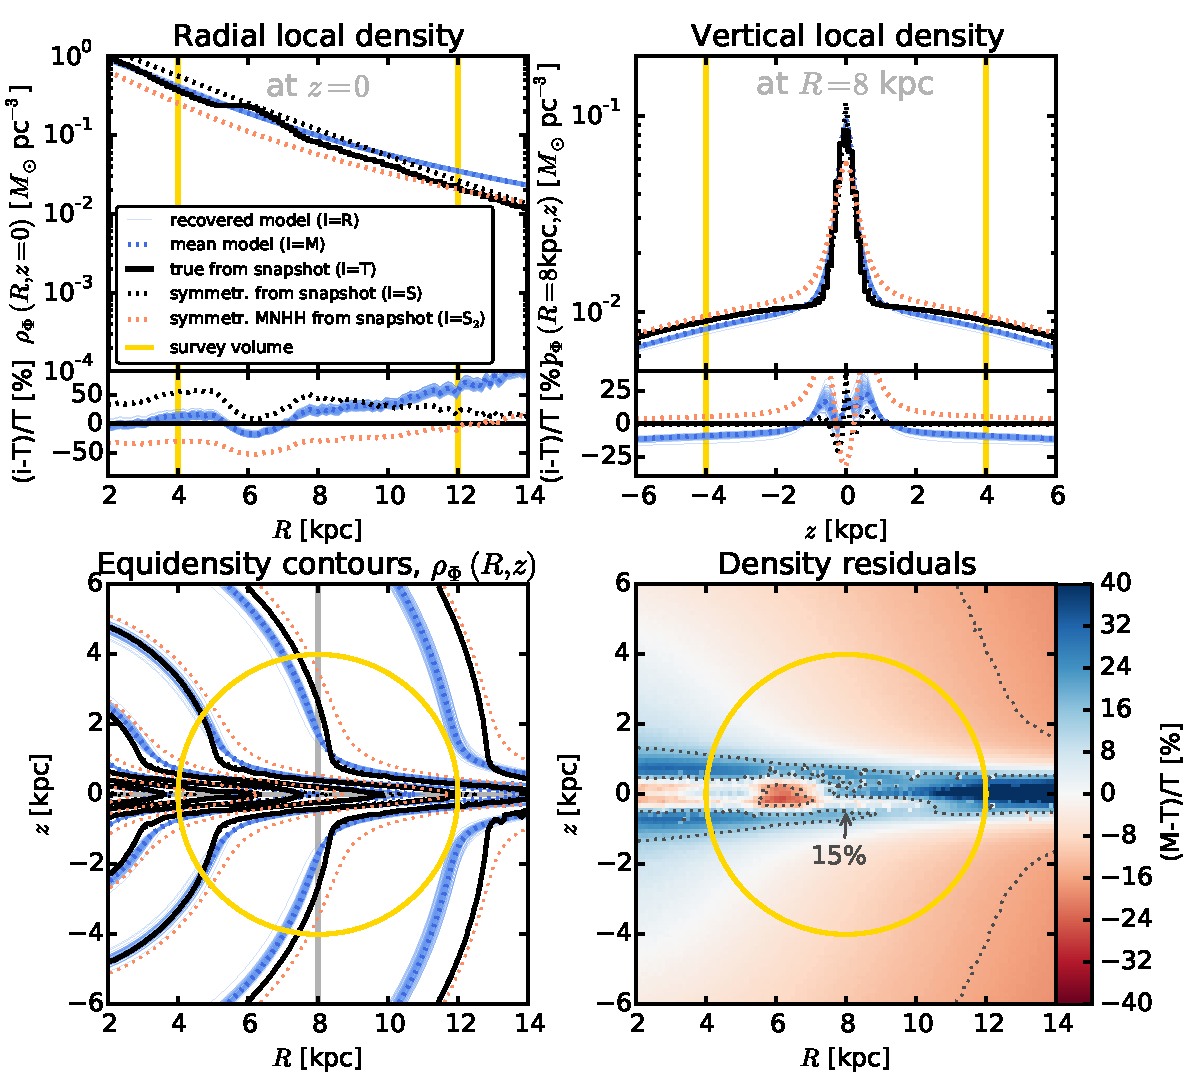
\includegraphics[width=\columnwidth]{fig/MNdHHdiffSph2_4kpc8Spiral_a_test1_density_overview.pdf}
\caption{Comparison of the true density distribution $\rho_{\Phi,\text{T}}$ in the galaxy simulation snapshot (solid black line, averaged over $\phi$) with the axisymmetric density distribution $\rho_{\Phi,\text{R}}$ recovered with \RM{} (solid blue lines) from $N_*=20,000$ stars in the survey volume \texttt{S8} with $r_\text{max}=4~\text{kpc}$ (yellow line). The first two panels show density profiles along $(R,z=0)$ and $(R=8~\text{kpc},z)$, together with the relative differences between true and recovered $\rho_{\Phi}$. The third panel displays equidensity contours of the matter distribution in the $(R,z)$ plane. Overplotted are also the overall axisymmetric \texttt{DEHH-Pot}'s $\rho_{\Phi,\text{S}}$ (dotted black line) (see Section \ref{sec:DEHH-Pot}) and the $\rho_{\Phi,\text{M}}$ of the recovered mean model in Table \ref{tbl:MNHHdiffSph2_4kpc8Spiral} (dotted blue line). The last panel shows the relative difference between the true $\rho_{\Phi,\text{T}}$ (averaged over all $\phi$) and the recovered mean model $\rho_{\Phi,\text{M}}$. Over wide areas even outside of the survey volume the relative difference is less than $15\%$. At $R\gtrsim8~\text{kpc}$ and $z\sim0$ it becomes apparent that the chosen potential model cannot perfectly capture the structure of the disk. However, in the plane of the disk and at smaller radii within the survey volume, where most of the stars are located, the model gives pretty good constraints on the density.  \Wilma{TO DO: Redo plot. Now I use the median of MCMC samples as best fit model.]} \Wilma{[TO DO: Make survey volume dark orange.]} \Wilma{[TO DO: Plot vertical profile from -5 to +5 only, to see disk better.]} \Wilma{[TO DO: Mention different potential model names in legend]} \HW{[TO DO: Maybe show the profiles not at R=8 and z=0, but at R=6 and z=$h_z$ or so.]} \HW{[TO DO: Decide if we want to include the local density (averaged over survey volume's wedge only) in this figure as well.]}}
\label{fig:4kpc8Spiral_density}
\end{figure}
%====================


\subsection{An axisymmetric galaxy model from \RM{}} \label{sec:results_part1}

In this section we will discuss the results of the \RM{} analysis of a single data set. This fiducial data set has $N_*=20,000$ stars that were drawn from the spherical volume with $r_\text{max}=4~\text{kpc}$ centered on a spiral arm at the ``solar'' radius $R=8~\text{kpc}$ shown as yellow sphere in Figure \ref{fig:simulation} (position \texttt{S8}). We use \RM{} to fit a single qDF (see Section \ref{sec:DF_model}) and the potential model \texttt{MNHH-Pot} consisting of a Miyamoto-Nagai disk, a Hernquist halo and a (fixed) Hernquist bulge introduced in Section \ref{sec:potential_model} to it. The best fit parameters are summarized in Table \ref{tbl:MNHHdiffSph2_4kpc8Spiral}. The circular velocity $v_\text{circ}(R_\odot)$ and halo fraction $f_\text{halo}$ are especially well recovered (compare to Table \ref{tbl:DEHH-Pot}).

\subsubsection{Recovering the stellar distribution} \label{sec:4kpc8Spiral_DF}

In Figure \ref{fig:4kpc8Spiral_DF_comparison} we compare the configuration phase-space distribution of the 20,000 stars that entered the \RM{} analysis as data with the best-fit stellar distribution, which is given by the action-based qDF and potential model found with \RM{}. We note that the spiral arms introduce very strong non-axisymmetries in the data, both in the spatial and the velocity distribution (especially in $v_R$, where a lot more stars move outside than inside as compared to an axisymmetric model). We therefore compare in Figure \ref{fig:4kpc8Spiral_DF_comparison} the data and fit separately for different spatial regions, $R>$ and $<8~\text{kpc}$ and $\phi<$ and $>5^\circ$. In the region where the spiral arm dominates (blue) the best fit \RM{} model is actually a very poor model. However, what the model underestimates in the spiral arm, it slightly overestimates in the other regions and is therefore indeed something like a good average model for the overall distribution. Especially the region at $R>8~\text{kpc}$ and $\phi<5^\circ$, where neither the spiral arm nor the inter-arm regions dominate strongly, is very well described by the model. This is remarkable because we had no indication beforehand that a single qDF might be at all a good enough model to describe the overall stellar distribution in the simulation snapshot. But it obviously does---apart from the spiral arm of course, which we had no chance to capture anyway.

\subsubsection{Recovering the gravitational potential} \label{sec:4kpc8Spiral_potential}

As shown in the previous section the best fit \RM{} model seems to reproduce the stellar phase-space distribution quite well. But is the corresponding potential close to the true potential? 

Figures \ref{fig:4kpc8Spiral_density} and \ref{fig:4kpc8Spiral_vcirc_surfdens} compare the true simulation snapshot potential and the axisymmetric \texttt{DEHH-Pot} from Table \ref{tbl:DEHH-Pot} with the best fit \texttt{MNHH-Pot} from the \RM{} analysis. In particular, Figure \ref{fig:4kpc8Spiral_density} illustrates the overall matter density distribution, Figure \ref{fig:4kpc8Spiral_vcirc_surfdens} the rotation curve, surface density profile and halo-to-disk ratio and Figure \ref{fig:4kpc8Spiral_forces} compares the true and recovered (median) gravitational forces at the position of each star in the data set. In Figure \ref{fig:4kpc8Spiral_vcirc_surfdens} we explicitely show the true simulation snapshot circular velocity both averaged over the whole $\Delta\phi=2\pi$ (black lines), and over the survey volume's maximum radial extent $\phi_0\pm \arcsin(r_\text{max}/R_0)$ (grey lines).

The recovery of density, surface density, circular velocity curve and disk-to-halo ratio is especially good in the region where most of the stars are located, around $R\sim~6\text{kpc}$ and in the plane of the disk. In large regions inside the survey volume, and even outside, the density is recovered to within 15\%. The circular velocity curve is even recovered to within 5\%, which is also approximately the extent of perturbation that the spiral arms cause with respect to a smooth rotation curve.

There is however a very small ($<1.5\%$) underestimation of $v_\text{circ}$ at larger radii. We suspect that this is a combination of a bias introduced by the spiral arms (see also discussion in Section \ref{sec:forces_bias}) and the choice of potential model (as a similar bias shows up in the \texttt{DEHH-Pot}). The overall surface density profile is a bit overestimated ($\sim 15\%$) at smaller radii; the reason is clearly the local spiral arm at $R\sim6~\text{kpc}$ with its higher surface density  and many stars entering the analysis, which bias the result and which was to be expected. At larger radii ($R\sim10-12~\text{kpc}$) the fit of radial local density and surface density profile is less good, which we account to the Miyamoto-Nagai disk having a shallower radial profile than an exponential disk, and not enough stars in this outer regions to give good constraints. The much stronger bias in the disk-to-halo ratio at larger radii is the result of a misjudgement of the halo scale length. As we will see later (see Figure \ref{fig:model_parameters}) we seem to need an even larger survey volume to have enough radial coverage to constrain the halo scale length properly. But again, where most of the stars are located, our \RM{} model is a very good average model for the true galaxy.

The aspect of the potential to which the stellar orbits are actually sensitive to, are the gravitational forces. In Figure \ref{fig:4kpc8Spiral_forces} we compare therefore the true force that each star in the data set feels ($F_{R,T}(*_i)$ and $F_{T,M}(*_i)$, calculated as sum of the individual contributions by each particle in the simulation and the analytic dark matter halo) with the force that the \RM{} median model predicts for each star ($F_{R,M}(*_i)$ and $F_{z,M}(*_i)$). We scale the difference between truth and model by a typical radial or vertical force at the given radius for which we use
\begin{eqnarray}
F_{R,\text{typ}}(R) &\equiv& v^2_{\text{circ},S}(R) / R\\
F_{z,\text{typ}}(R) &\equiv& F_{z,S}(R,z=h_r),
\end{eqnarray}
where $v_{\text{circ},S}$ and $F_{z,S}$ are the circular velocity and vertical force evaluated in the ''true symmetric'' \texttt{DEHH-Pot} in Table \ref{tbl:DEHH-Pot}. As typical vertical force at a given radius we use the vertical force evaluated at the scale height $h_z=0.17~\text{kpc}$ of the disk, because we found that 
\begin{eqnarray*} 
&&\langle |F_{z,S} (*_i)| (R) \rangle \\
&\lesssim& \langle |F_{z,T}(*_i)|  (R) \rangle\\
&\lesssim& F_{z,S}(R,z=h_z) \\
&\lesssim& \langle J_z(*_i) \times \Omega_z(*_i) / h_r \rangle (R),
\end{eqnarray*}
where, e.g., $\langle |F_{z,T}(*_i)|  (R) \rangle$ denotes the mean of the absolute value of the true vertical force of all stars at radius $R$, and $J_z \times \Omega_z \sim \langle E_z \rangle$ is something like the mean vertical energy of a stellar orbit. Figure \ref{fig:4kpc8Spiral_forces} shows therefore
\begin{eqnarray}
\Delta F_R(*_i) \equiv \frac{|F_{R,M}(R_i,z_i)| - |F_{R,T}(x_i,y_i,z_i)|}{F_{R,\text{typ}}(R_i)}\label{eq:delta_FR}\\
\Delta F_z(*_i) \equiv \frac{|F_{z,M}(R_i,z_i)| - |F_{z,T}(x_i,y_i,z_i)|}{F_{z,\text{typ}}(R_i)}\label{eq:delta_Fz}
\end{eqnarray}
for each star. The recovery is as expected: The true vertical force is stronger in the spiral arms (due to the higher surface density) and weaker in the inter-arm regions as compared to the axisymmetric best fit model. The radial force is well recovered where the majority of the stars are located, i.e. in the wide inter-arm regions and in the peaks of the spiral arms. Misjudgments happen in the wings of the spiral arms: The true radial force (i.e., the pull towards the galactic center) is stronger at the outer edge/leading side of the spiral arm because of the additional gravitational pull towards the massive spiral arm, and for the same reason weaker at the inner edge/trailing side. Overall the recovered \RM{} model appears to be a good mean model, averaging over spiral arms and inter-arm regions.


%====================
\begin{figure*}[!htbp]
\centering
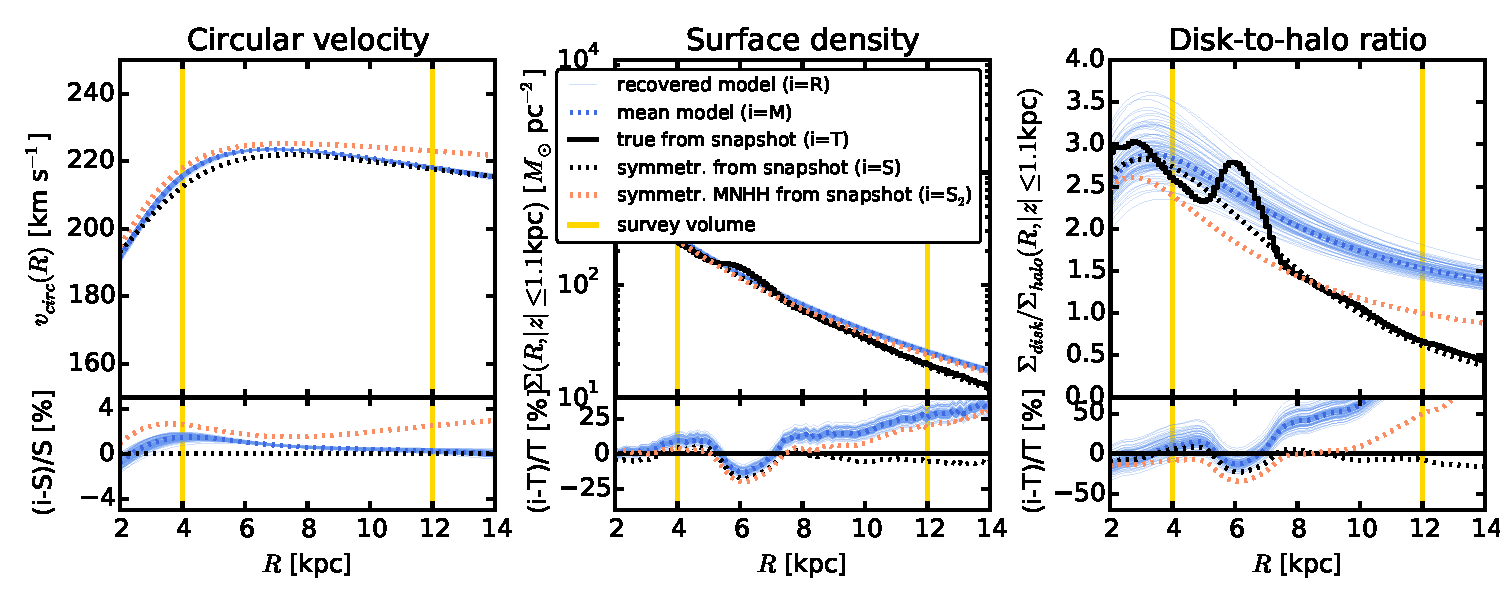
\includegraphics[width=0.9\textwidth]{fig/MNdHHdiffSph2_4kpc8Spiral_a_test1_vcirc_surfdens_overview.pdf}
\caption{Comparison of the circular velocity curve, surface density profile within $|z|\leq1.1~\text{kpc}$ and disk-to-halo ratio of the surface density along $R$ for the true potential of the galaxy simulation snapshot (solid black line for the global average over $\phi_0\pm\pi$; solid grey line for the local average over $\phi_0\pm \arcsin(r_\text{max}/R_0)$) and the axisymmetric model potential recovered with \RM{} (solid blue lines) (see Section \Wilma{[TO DO]}). Overplotted are also the profiles of the symmetrized ''true'' \texttt{DEHH-Pot} (dotted black line) (see Section \ref{sec:DEHH-Pot} and Table \ref{tbl:DEHH-Pot}) and the recovered mean model (dotted blue line) (see Table \ref{tbl:MNHHdiffSph2_4kpc8Spiral}). The circular velocity curve is recovered to less than $5\%$, especially at larger radii. For the surface density and disk-to-halo ratio \RM{} recovers the truth at radii $\lesssim 8~\text{kpc}$. The deviations at larger radii are connected to the discrepancies in the density in Figure \ref{fig:4kpc8Spiral_density}. \Wilma{[TO DO: Add grey curve for disk to halo ratio.]} \Wilma{[TO DO: Make survey volume dark orange.]} \Wilma{[TO DO: Mention different potential model names in legend]}}
\label{fig:4kpc8Spiral_vcirc_surfdens}
\end{figure*}
%====================

%====================
\begin{figure*}[!htbp]
\centering
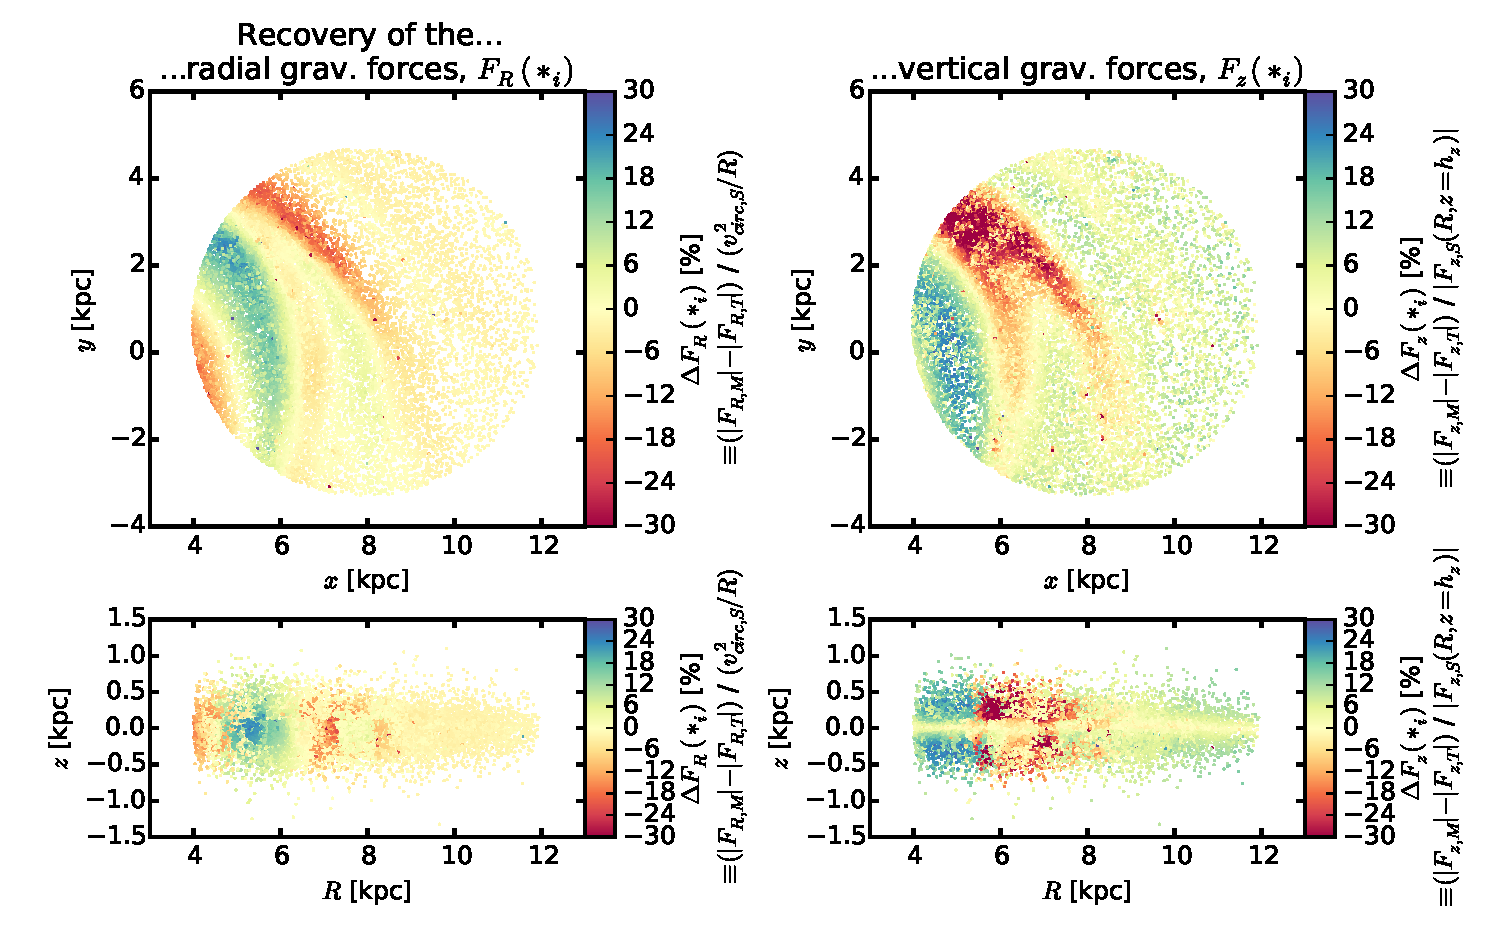
\includegraphics[width=0.7\textwidth]{fig/MNdHHdiffSph2_4kpc8Spiral_a_test1_forces_overview_6.pdf}
\caption{Comparison of the true gravitational forces with the forces estimated from the \RM{} best fit potential in Table \ref{tbl:MNHHdiffSph2_4kpc8Spiral} at the $(x,y)$ (upper panels) and $(R,z)$ positions (lower panels) of the stars that entered the analysis. In particular we colour-code the positions of the stars according to the radial (left panels) and vertical (right panels) force residuals scaled by a typical force, i.e., $\Delta F_R(*_i)$ and $\Delta F_z(*_i)$ in Equations \eqref{eq:delta_FR}-\eqref{eq:delta_Fz}. Red means an underestimation of the (absolute value of the)  true force---which is the case for the radial force in the leading sides of the spiral arms and the vertical force within the spiral arms, which cannot be reproduced ---and blue correspondingly an overestimation of the force. Overall the radial forces are very well recovered, which is related to the well recovery of the circular velocity curve in Figure \Wilma{???}. There are more problems with the vertical force, which is related to the higher surface densities in spiral arms which slightly biases the overall \RM{} model. \Wilma{[TO DO: Might be, that I have to re-calculate the forces for some of the stars. Write Test that tests if force >1e10 and then recalculates those forces.]}}
\label{fig:4kpc8Spiral_forces}
\end{figure*}
%====================


\subsubsection{Recovering the action distribution}

In Sections \ref{sec:4kpc8Spiral_DF} and \ref{sec:4kpc8Spiral_potential} we have demonstrated the goodness of fit in the configuration space of the data, and of the recovered gravitational potential. What \RM{} is actually fitting is however the distribution in action space. Figure \ref{fig:4kpc8Spiral_actions} compares the data and the model action distribution given the best fit \text{MNHH-Pot} in Table \ref{tbl:MNHHdiffSph2_4kpc8Spiral}. (We only use this axisymmetric potential to estimate the actions as they enter the fit, and do not calculate the true actions in the true potential.)

We note that the radial and vertical action distribution fits indeed quite well; the axisymmetric model however contains much more stars on close to circular orbits $(J_R \sim 0,J_z \sim 0)$ than the simulation does. In the data set there is an excess of stars in the galactic plane $(J_z\sim0)$ that have more eccentric orbits  than the axisymmetric model would have. In Figure \ref{fig:DF_densres} we have marked the radial extent of the stronger spiral arm with dotted lines ($R_\text{spiral} \in [5.6,6.8]~\text{kpc}$), and over-plotted the corresponding angular momenta $L_z = R_\text{spiral} \times v_\text{circ}(R_\text{spiral})$ in Figure \ref{fig:4kpc8Spiral_actions} as a rough estimate where in action space we expect the stars of this spiral arm. It is again obvious that this spiral arm contains (i) more stars in general and (ii) more stars with eccentric orbits  $(J_R>0)$ which are (iii) located mostly close to the plane $(J_z\sim0)$, as compared to the axisymmetric model. All of this confirms our expectations for orbits in a spiral arm. 

This exercise of comparing the data and the model actions in a best-fit axisymmetric potential should be performed for a future application to data in the Milky Way as well. It could help to learn about the approximate orbits that stars move on in real spiral arms and to subsequently construct orbit distribution functions for spiral arms.


\begin{figure}[!htbp]
\centering
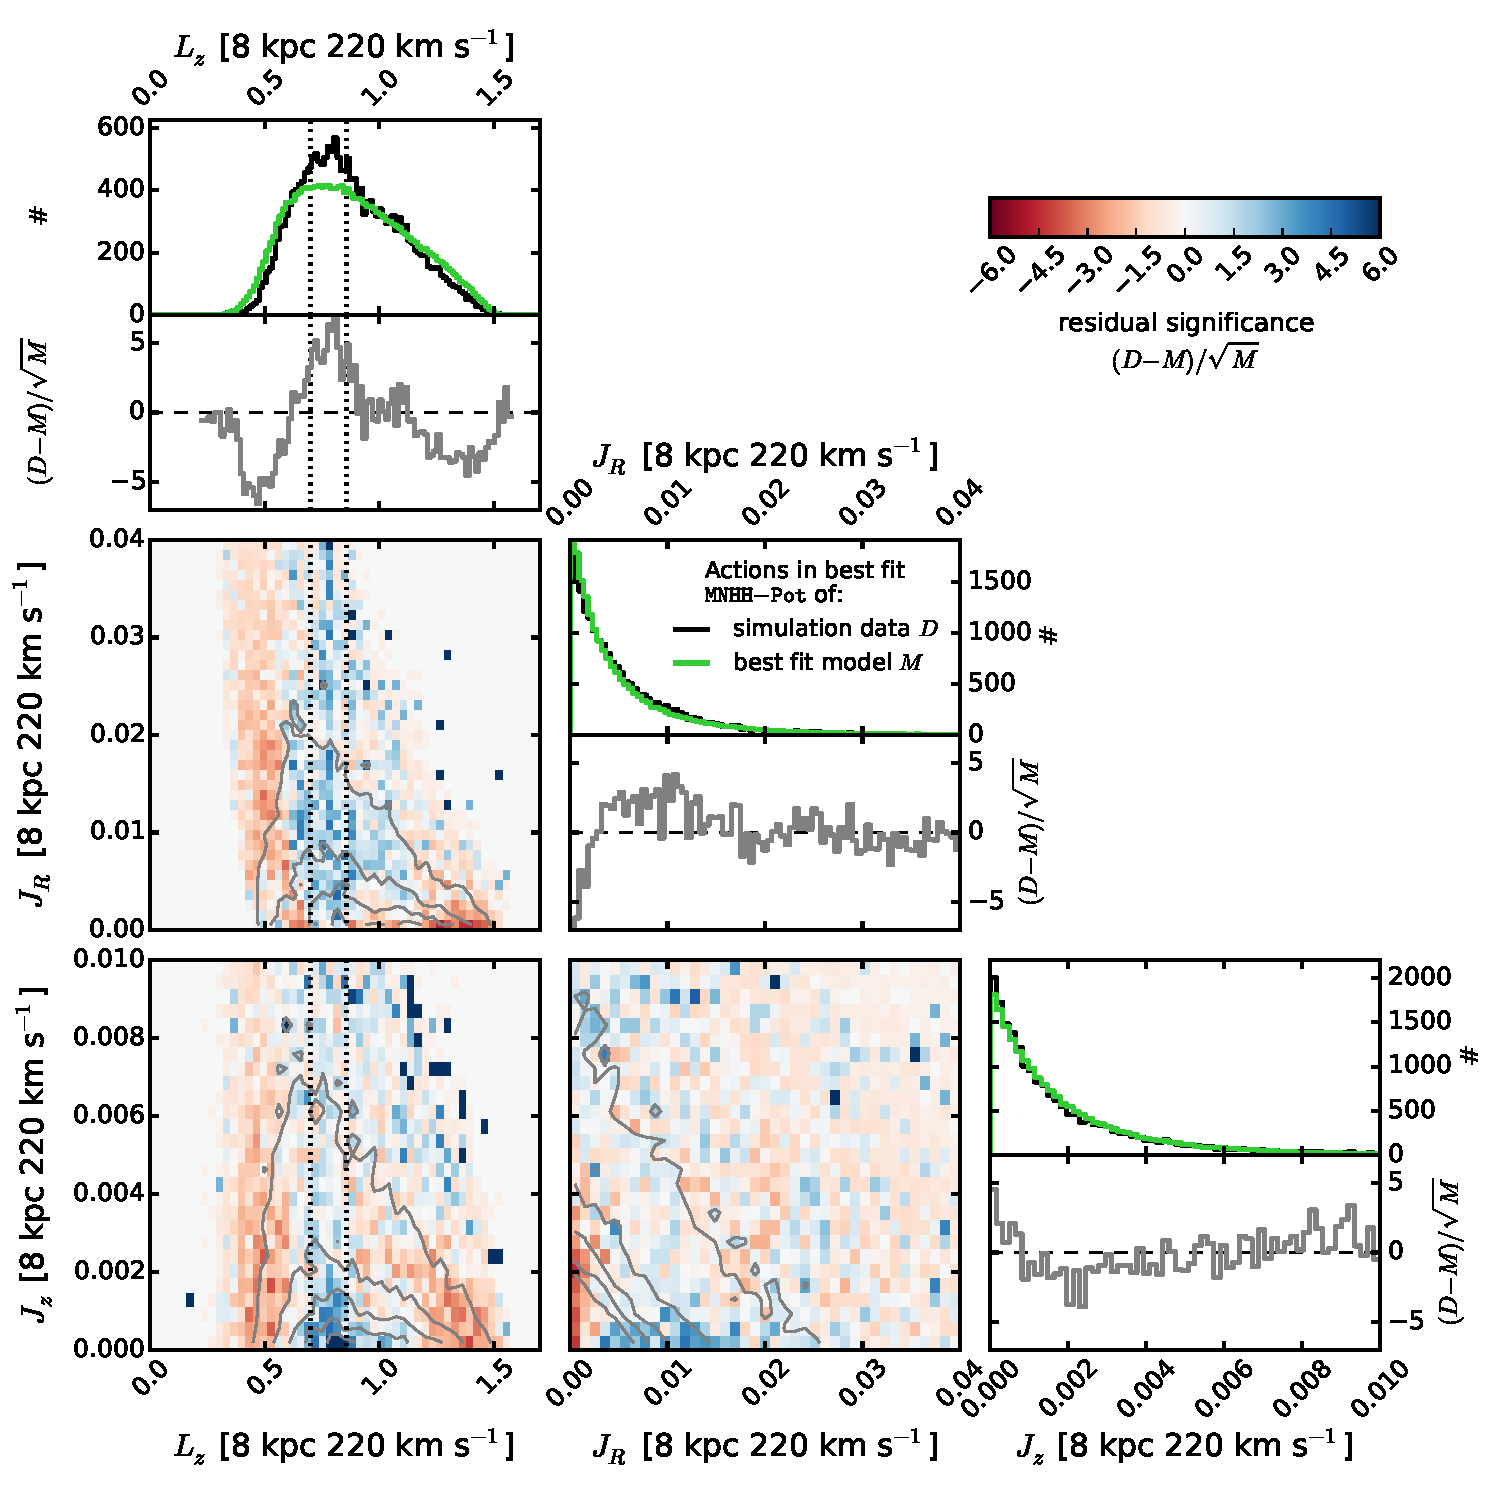
\includegraphics[width=\columnwidth]{fig/MNdHHdiffSph2_4kpc8Spiral_a_data_bestfit_residuals_only_actions.pdf}
\caption{Comparison of the stellar action distribution of the data set $D$ used in the analysis and the recovered axisymmetric stellar distribution $M$ (see Figure \ref{fig:4kpc8Spiral_DF_comparison} for the distribution in configuration space). All actions, of data set and best fit distribution, where calculated in the best fit \texttt{MNHH-Pot} in Table \ref{tbl:MNHHdiffSph2_4kpc8Spiral}. The upper panel in each column compares the 1D histograms of the  angular momentum $L_z$, the radial action $J_R$ and the vertical action $J_z$ of both data and best fit. The other 1D and 2D distributions show the residual significance $(D-M)/\sqrt{M}$. The 2D residuals are over-plotted with equidensity contours of the data $D$'s 2D action distribution. In Figure \ref{fig:DF_densres} we have marked the approximate radial extent of the stronger spiral arm with black dotted lines ($R_\text{spiral} \in [5.6,6.8]~\text{kpc}$); the dotted lines in the $L_z$ distributions in this figure correspond to $L_z = R_\text{spiral} \times v_\text{circ}(R_\text{spiral})$. This comparison gives a first impression of how he approximate action distribution in spiral arms might look like. An open task that the Galactic dynamical modelling community faces in the future, is to construct orbit distribution functions for spiral arms. \Wilma{[TO DO: Calculate reference data new. Now I use the median of MCMC samples as best fit model.]} \Wilma{[TO DO: Add in legend that simulation data was calculated in best fit potential too.]}}
\label{fig:4kpc8Spiral_actions}
\end{figure}

\Jo{[TO DO: Jo writes: "If you make the equivalent of Figure 7 for fits that are especially good and those that are especially bad, is the difference between the qDF prediction and the data that went into the analysis very different? If so, that might be nice to point out and then say that we will investigate this in later work."]}

\subsection{The influence of spiral arms in \RM{} modelling} \label{sec:results_part2}

In the previous section we showed that for a large enough survey volume ($r_\text{max}=4~\text{kpc}$) \RM{} can construct a good average axisymmetric potential (and DF) model for a galaxy with spiral arms. In the following we want to investigate how this modelling success depends on the position and the size of the survey volume within the galaxy and with respect to the spiral arms.

\subsubsection{Test suite}

We center our test survey volumes at the positions marked in Figures \ref{fig:simulation} and \ref{fig:spiral_arm_kappa} (see also Table \ref{tbl:volume_positions}) and consider volume sizes with $r_\text{max} \in [0,1,2,3,4,5]~\text{kpc}$ for $R_0 = 8~\text{kpc}$ and $r_\text{max} \in [0,1,2,3,4]~\text{kpc}$ for $R_0 = 5~\text{kpc}$ (to avoid the galactic center). As demonstrated in Figure \ref{fig:spiral_arm_kappa} the spiral arm strength is very different in these test volumes. Each data set that we draw from the simulation contains a random selection of $N_*=20,000$ stars inside the given spherical volume and we fit a single qDF and \texttt{MNHH-Pot} to it. 

\subsubsection{Discussion of the model parameter recovery} \label{sec:parameter recovery}

Figure \ref{fig:model_parameters} shows the best fit parameters for the different \RM{} analyses. We also overplot the parameters of the reference \texttt{DEHH-Pot} from Table \ref{tbl:DEHH-Pot}. Overall the statistical random errors on the parameter recovery are very small for $N*=20,000$ and possible systematic errors dominate. 

There are only a few exceptions ($r_\text{max}=1~\text{kpc}$ at \texttt{I5}, $r_\text{max}=2~\text{kpc}$ at \texttt{I8}), which we will discuss later.

Let's first consider the parameters of the gravitational potential: All volumes recover $v_\text{circ}(R_\odot)$ within a few $\text{km s}^{-1}$; in the largest volumes, where the circular velocity curve is probed over several $\text{kpc}$ the estimate is the most accurate. The halo fraction $f_\text{halo}$ of the radial force at the Sun is very well recovered, especially for $r_\text{max}\gtrsim 2~\text{kpc}$. The estimate that we get for the best fit Miyamoto-Nagai disk scale height $b_\text{disk}$ seems to be also approximately independent of the size of the volume. We can even recover the true halo scale length $a_\text{disk}$, however only for a volume as large as $r_\text{max}=5\text{kpc}$. The models at $r_\text{max}=500~\text{kpc}$ appear to be too small to constrain the halo at all. Smaller volumes that underestimate $a_\text{halo}$ get slightly larger estimates for the disk scale length $a_\text{disk}$ and the overall radial density slope is then probably closer to the truth, even if the individual parameters are not. Outliers can be often explained by having a look at the data: The large disk scale length recovered from the $r_\text{max}=2~\text{kpc}$ volume at \texttt{S5} for example mirrors the comparably flat matter distribution caused by two spiral arms close together and dominating the volume (see the large $\sigma_\kappa$ for this analysis in the right panel of Figure \ref{fig:spiral_arm_kappa}, and Figure \ref{fig:2kpcSuite}). 

The right column of Figure \ref{fig:model_parameters} compares the recovered qDF parameters for the different survey volumes with the qDF parameters we got from fixing the potential model to the \text{expHH-Pot} and fitting the qDF only in a $r_\text{max}=5~\text{kpc}$ volume. Even though the qDF parameters for small volumes are widely different for different positions within the galaxy, they all approach the values recovered with the \texttt{DEHH-Pot} for larger volumes. There seems therefore to be indeed an overall best-fit qDF describing the average tracer distribution in the galaxy's disk. The only difference is in the $h_{\sigma,z}$ parameter, where the models with free \texttt{MNHH-Pot} recover a slightly larger value than the models using the known \texttt{expHH-Pot}. The reason is that the Miyamoto-Nagai disk has a different radial profile than the double exponential-disk (see Figure \ref{fig:4kpc8Spiral_density}), which leads to a less steep radial decline in the vertical forces and therefore mean vertical orbital energies $\langle E_z \rangle \sim \nu \times J_z$ and therefore to a slightly longer $h_{\sigma,z}$ scale length. In general, volumes centered on spiral arms have larger velocity dispersion parameters $\sigma_{R,0}$ and $\sigma_{z,0}$ as compared to volumes at the same radius $R_0$ but centered on an inter-arm region, and the volumes at $R_0=5~\text{kpc}$ with their stronger spiral arms have larger velocity dispersions than those at $R_0=8~\text{kpc}$---which is what we expect. Most volumes recover similar tracer scale lengths $h_R\sim2.5\pm0.5~\text{kpc}$ close to the known disk scale length; only the volumes centered on the inter-arm region at $R_0=8~\text{kpc}$ (position \texttt{I8}) recover much longer $h_R$. This might be related to the fact, that volumes at \texttt{I8} are dominated by a especially large inter-arm region.

There are a few survey volumes for which the recovered parameters show some peculiarities: The models from volumes with $r_\text{max}=1~\text{kpc}$ at \texttt{I5} and $r_\text{max}=2~\text{kpc}$ at \texttt{I8} reject the dark matter halo completely, i.e., $f_\text{halo}=0$. The corresponding halo scale lengths $a_\text{halo}$ are therefore also pretty unconstrained, while the corresponding disk scale heights $b_\text{disk}$ are grossly overestimated to account for the missing contribution of the spherical halo. We have investigated the reason for this fitting result and found, that for the way how the spiral arms affect the circular velocity curve in these volumes, the recovered models with unusual radial profiles are indeed a better description for the data (see Figure \ref{fig:1kpcSuite}-\ref{fig:2kpcSuite}). Also, while most analyses average the vertical forces radially over the spiral arms(see Figures \ref{fig:4kpc8Spiral_forces}, lower right panel), for these analyses the averaging happens vertically, i.e., at some height above the plane \Wilma{[TO DO: check if this is approximately the scale height]} the model's vertical forces are equally good at all radii (in spiral arms and between), while at small and large $|z|$ the model is bad. \RM{} therefore found a good average fit model also for the stars in these volumes. 

\Wilma{[TO DO: Make the same diagnostic plots for 1kpc5Void as for 2kpc8Void and check that my explanation of fhalo=0 in this text is indeed correct.]}


%====================
\begin{figure}[!htbp]
\centering
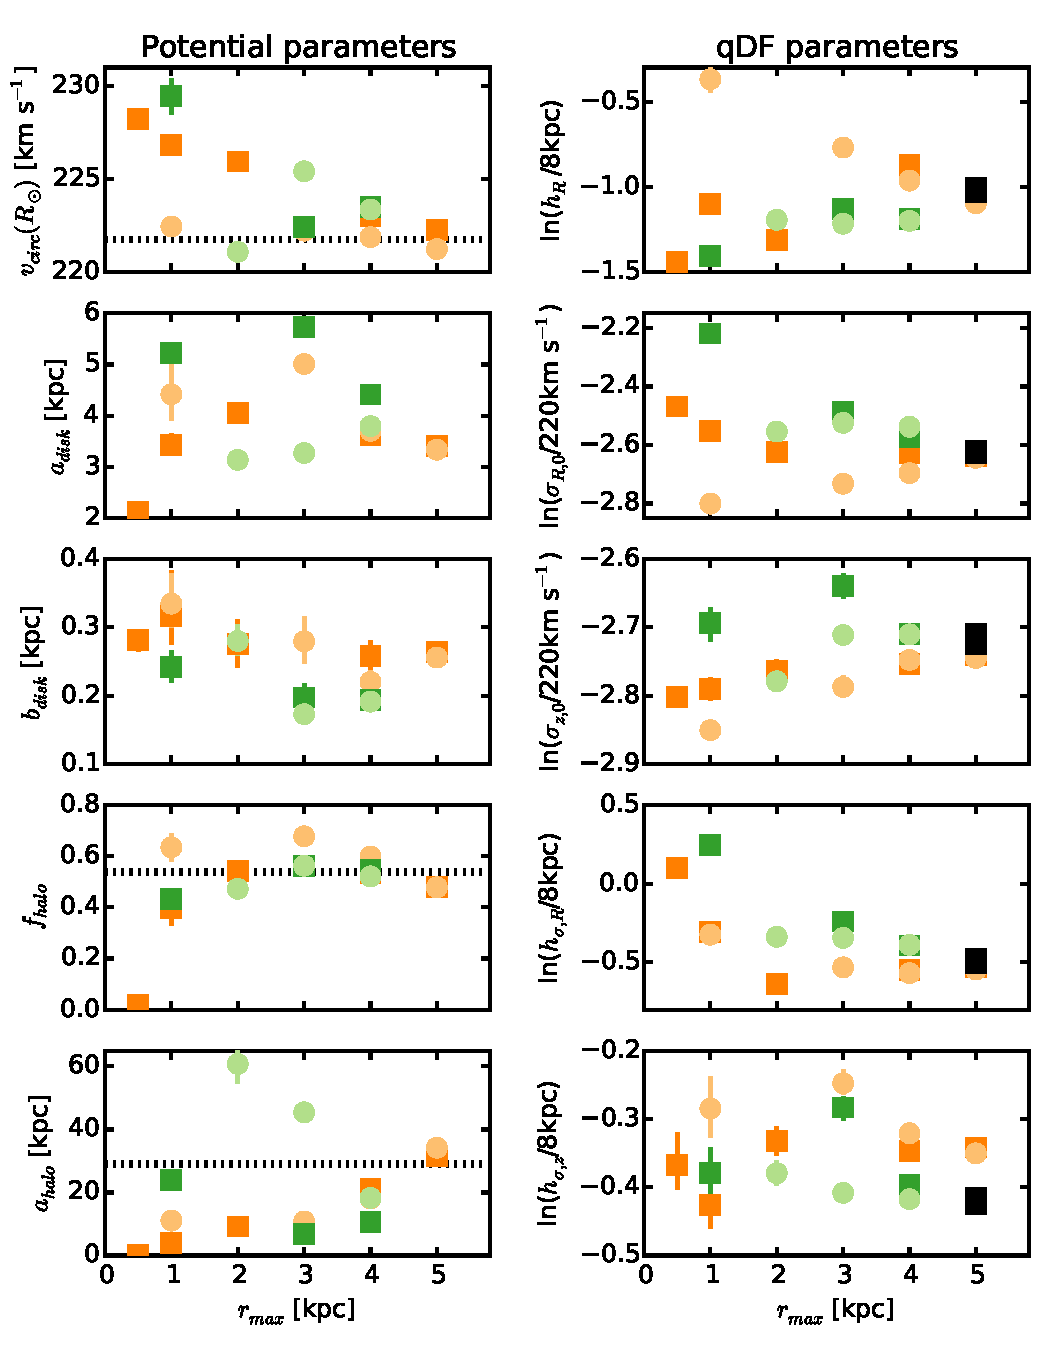
\includegraphics[width=\columnwidth]{fig/MNdHHdiffSph2_violins.pdf}
\caption{\Wilma{[TO DO: Check that caption is still fine.]} Overview over the model parameter estimates (\texttt{MNHH-Pot} parameters on the left, qDF parameters on the right) recovered with \RM{} from data sets drawn from the simulation snapshot at different positions in the galaxy (colour-coded) and of different size ($r_\text{max}$ as indicated on the $x$-axis). The black dotted line shows the known model parameters from the \texttt{DEHH-Pot} in Table \ref{tbl:DEHH-Pot} (the Miyamoto-Nagai disk parameters $a_\text{disk}$ and $b_\text{disk}$ are related but not directly comparable to an exponential disk scale length and height). The black squares denote the qDF parameters we recovered by fixing the potential to the \texttt{DEHH-Pot}, centering a survey volume with $r_\text{kpc}=5$ on the spiral arm at $R=8~\text{kpc}$, and fitting the qDF only. A survey volume with a radial coverage as large as $r_\text{max}=5~\text{kpc}$ is required to properly recover the ''true'' model parameters. \Wilma{TO DO: Preliminary. Add more results. Make sure that the "true" potential parameters are the final version.} \Wilma{[TO DO: Add additional y-axis on right side of plot with non-log values.]}}
\label{fig:model_parameters}
\end{figure}
%====================

\subsubsection{Recovery of the gravitational forces depending on the size of the survey volume}\label{sec:forces_bias}

In the previous section we found that the potential and qDF parameters recovered from different survey volumes can differ by quite a lot. While the differences can be qualitatively explained, it is not clear yet how good the corresponding potential constraints actually are in a quantitative sense. To test this we calculate again $\Delta F_R(*_i)$ and $\Delta F_z(*_i)$ from Equations \eqref{eq:delta_FR}-\eqref{eq:delta_Fz} at the position of each star $*_i$ in each data set (see also Figure \ref{fig:4kpc8Spiral_forces}). From the corresponding histograms we derive the median and the $15.87th$ and $84.13th$ percentiles and show them in the left panels of Figure \ref{fig:forces_bias}. We chose this diagnostic because the forces at the positions of the stars are the quantities of the potential to which our modelling is sensitive to.

In addition it is interesting to see, how good a recovered potential describes the overall gravitational potential of the galaxy, i.e. its "predictive power". We introduce another diagnostic, that uses a cylindrical grid centered on the respective positions in Table \ref{tbl:volume_positions}, having always a radius of $r_\text{max}=5~\text{kpc}$ and a height of $z=1.5~\text{kpc}$ both above and below the plane.  In the $(x,y)$ plane the regular grid points have a distance of $0.25~\text{kpc}$ and in $z$ they have a distance of  $0.125~\text{kpc}$ to better sample the thin disk. (We throw out grid points close to the galactic center with $R<0.125~\text{kpc}$, however.) \HW{[comment: This was decided completely arbitraryly. I guess we can think of a slightly different grid, that is more motivated.]} We then evaluate at the position $g_j \equiv (x_j,y_j,z_j)$ of each regular grid point the force residuals
\begin{eqnarray}
\Delta F_R(g_j) \equiv \frac{|F_{R,M}(R_j,z_j)| - |F_{R,T}(x_j,y_j,z_j)|}{F_{R,\text{typ}}(R_j)} \label{eq:delta_FR_grid}\\
\Delta F_z(g_j) \equiv \frac{|F_{z,M}(R_j,z_j)| - |F_{z,T}(x_j,y_j,z_j)|}{F_{z,\text{typ}}(R_j)},\label{eq:delta_Fz_grid}
\end{eqnarray}
analogous to Equations \eqref{eq:delta_FR}-\eqref{eq:delta_Fz}. The two panels on the right in Figure \ref{fig:forces_bias} show the [$15.87th$,$84.13th$] percentile range and the median of the grid points' distribution in $\Delta F_R(g_j)$ and $\Delta F_z(g_j)$.


%====================
\begin{figure*}[!htbp]
\centering
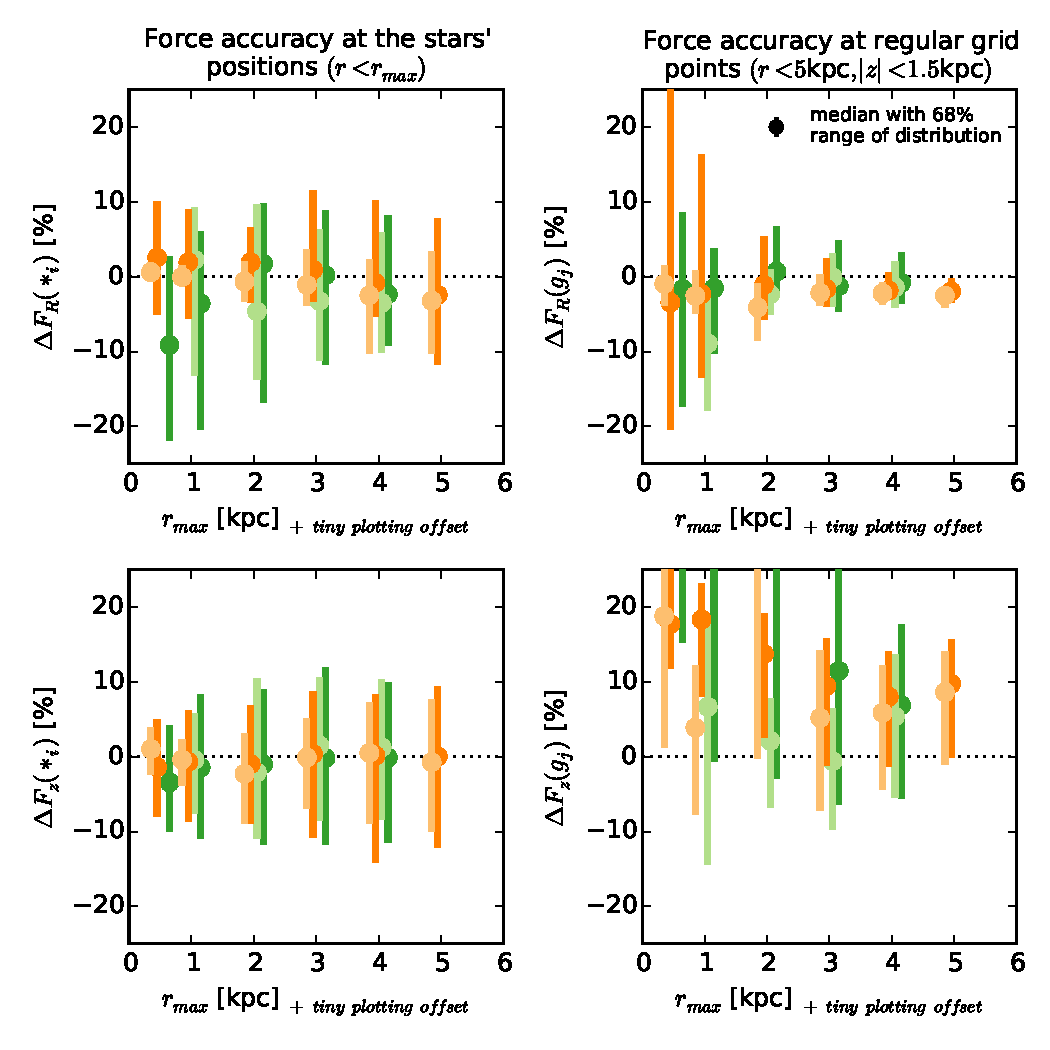
\includegraphics[width=0.6\textwidth]{fig/MNdHHdiffSph2_bias_in_forces_recovery_2.pdf}
\caption{Accuracy of the radial (upper panels) and vertical (lower panels) gravitational forces recovered with \RM{} from the suite of data sets introduced in Section \ref{sec:suite_parameters}, depending on the size $r_\text{max}$ of the survey volume. The left panels investigate how well \RM{} recovers the forces for the ensemble of stars in the data set ($\Delta F_{R/z}(*_i)$ in Equations \eqref{eq:delta_FR}-\eqref{eq:delta_Fz}) and the right panels test the ''predictive power'' of each of the data sets' best-fit potential by showing how well the forces are recovered at regular grid points in a large cylinder of $r_\text{max}=5~\text{kpc}$ and height $|z|=1.5~\text{kpc}$ around the survey volumes center ($\Delta F_{R/z}(g_j)$ in Equations \eqref{eq:delta_FR_grid}-\eqref{eq:delta_Fz_grid}). For each distribution of $\Delta F_{R/z}(*_i)$ and $\Delta F_{R/z}(g_j)$ we show here the median as dot with the  [$15.87th$,$84.13th$] percentile range as bar. We find that the forces are very well recovered at the positions of the stars independent of the size of the volume. The spiral arms introduce some biases in the overall recovered potential and we need at least a survey volume of $r_\text{max}=3~\text{kpc}$ to get a potential with a reasonable ''predictive power''. \Wilma{[TO DO: Make sure all final analyses are in this plot.]} \Wilma{[TO DO: Add legend to plot.]} \HW{[TO DO: Jo suggested to make the right lower plot for slices at different heights, because it is very likely that most of the misjudgement is at high z. Alternatively we could use a different reference volume that's not going up to 1.5kpc but maybe only up to 3-4 scale heights?]}}
\label{fig:forces_bias}
\end{figure*}
%====================

The first and most important thing to learn from Figure \ref{fig:forces_bias} is, that we get very close to recovering the true forces at the positions of the stars in the survey volume, no matter how large the survey volume is.

Second, if we consider not the stars inside the survey volume, but the spatial average of the forces in the fixed cylindrical volume ($r_\text{max}=5~\text{kpc}$, as described above), the radial forces are overall very well recovered, especially for large survey volumes. There is however a overestimation of $\sim5-20\%$ in the vertical forces (depending on volume size and position) which is induced by the spiral arms (see explanation below).

Third, the constraints we get on the spatially averaged forces inside $r<5~\text{kpc}$ are almost as good for the survey volume of $r_\text{max}=3~\text{kpc}$ as compared to survey volumes of $r_\text{max}=4$ or $5~\text{kpc}$. If we had to decide between a $r_\text{max}=3~\text{kpc}$ volume with good data quality and a larger volume with worse data quality, we would loose nothing in terms of force recovery when using the smaller volume. (Only the halo scale length might not be as well constrained, see Figure \ref{fig:model_parameters}).

Now let's discuss the reason for the biases that we observe. The peak of the distribution in $\Delta F_R(*_i)$ and $\Delta F_R(g_j)$ is slightly biased towards an underestimation of $|F_{R,M}|$ in our \RM{} models. We think the explanation is the following: Spiral arms are very thin. If a spiral arm crosses the observation volume both its leading side (at large radii) and its trailing side (at small radii) are also in the volume. Stars in the trailing side feel a lower gravitational pull towards the galaxy center than they would if there was no spiral arm. Because there are in general more stars at smaller radii, the \RM{} fit is slightly biased to reproduce in general slightly weaker radial forces (see also Figures \ref{fig:4kpc8Spiral_vcirc_surfdens} and \ref{fig:4kpc8Spiral_forces}).

The peak of $\Delta F_z(*_i)$ is approximately at 0, while the peak of $\Delta F_z(g_j)$ is strongly biased towards an overestimation of $|F_{z,M}|$. There are much more stars in the spiral arms than in the inter-arm regions, and the stars in the spiral arm feel stronger vertical forces because of the higher disk mass. \RM{} finds a model that in general has much stronger vertical forces than expected for a smooth potential. While the actual vertical forces that the many stars in the spiral arms feel are very well recovered, it becomes obvious when looking at the grid points regularly distributed in space, that the \RM{} vertical forces are much stronger. As expected the overestimation is especially strong ($\sim 20 \%$) for small survey volumes dominated by spiral arms, while small volumes dominated by an inter-arm region result in much better estimates for the spatially averaged $F_z(g_j)$ ($\sim5\%$ bias). Large volumes lie somewhere in between (bias of $\sim10\%$).

Because the stellar number asymmetry in the trailing vs. leading sides of spiral arms is much smaller than the stellar number asymmetry in spiral arm vs. inter-arm region, the bias is visible in the distribution of $\Delta F_R{*_i}$ (the $F_R$ recovery is biased only by a few stars which leads to a bias which is visible for the majority of stars) and not in $\Delta F_z(*_i)$ (the majority of stars biases the fit and we therefore recover $F_z$ also for the majority of stars), but becomes really pronounced for $\Delta F_z{g_j}$ (the inter-arm regions dominate when averaging spatially which leads to a large overestimation of $F_z$ spatially) and stays small for $\Delta F_R{g_j}$ (trailing and leading sides of spiral arms are similarly important when averaging spatially so it becomes visible that the bias is actually not that big).

\Jo{[TO DO: Jo writes: "I do think it would be good to look a little more deeply in why the predictive $F_Z$ fails so much by looking at where most of the difference is (close to the plane or far away from it)." $\longrightarrow$ TO DO: Include figure Fg vs z and discuss it in text.]}

%====================
\begin{figure}[!htbp]
\centering
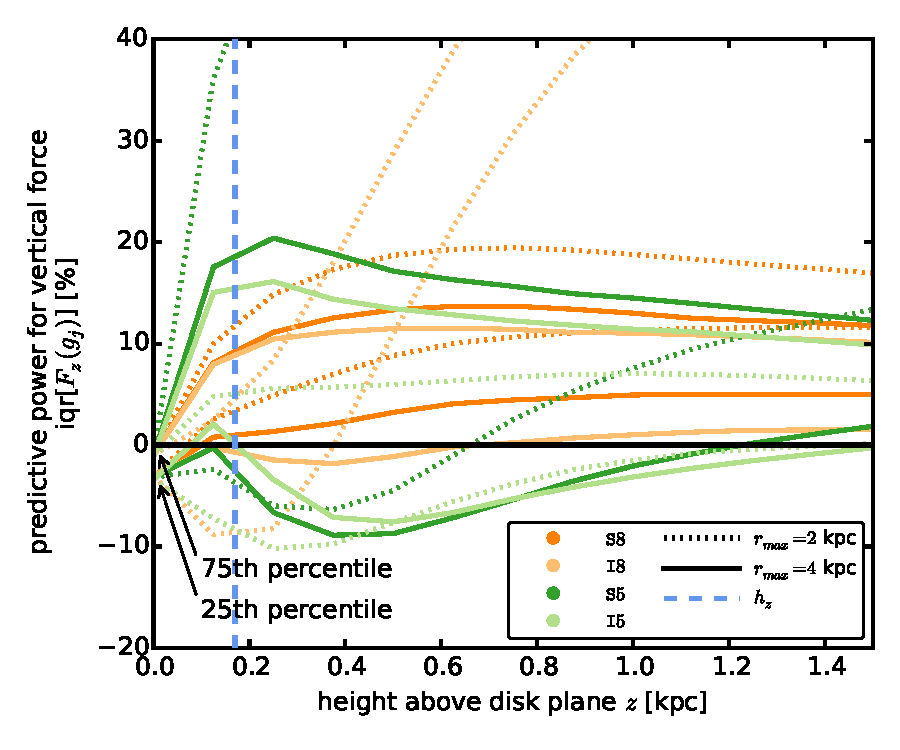
\includegraphics[width=\columnwidth]{fig/MNdHHdiffSph2_Fg_vs_z.pdf}
\caption{\Wilma{[TO DO]}}
\label{fig:??}
\end{figure}
%====================


\subsubsection{Influence of spiral arms on the recovery of the gravitational forces} \label{sec:spiral_arms_and_forces}

The Figure \ref{fig:forces_bias} in Section \ref{sec:forces_bias} gave an overview over the accuracy of the gravitational forces recovery for our whole suite of data sets depending on the size of the different survey volumes. In the following we want to relate the same quantities, i.e., local force recovery at the positions of the stars that entered the analysis (see Equations \eqref{eq:delta_FR}-\eqref{eq:delta_Fz}) and power of a recovered model to predict the forces in a fixed large volume (see Equations \eqref{eq:delta_FR_grid}-\eqref{eq:delta_Fz_grid}), to the actual strength and dominance of spiral arms in the respective survey volumes (see Section \ref{sec:spiral_arm_kappa}). In Figure \ref{fig:std_kappa_vs_frac10_stars} we find a connection between the local force recovery and the relative spiral contrast, and Figure \ref{fig:mean_kappa_vs_frac10_grid} shows a trend that the ''predictive power'' of the recovered model depends on the dominance of a spiral arm in the survey volume. The former was to be expected, but the latter is a very interesting result.


Let's have a closer look at Figure \ref{fig:std_kappa_vs_frac10_stars}, where we relate Equations \eqref{eq:delta_FR}-\eqref{eq:delta_Fz} (see also Figure \ref{fig:forces_bias}, left panels) to Equation \eqref{eq:std_kappa} (see also Figure \ref{fig:spiral_arm_kappa}, right panel). The average fraction of stars for which the recovery of radial or vertical force is bad (i.e., larger than 10\%) decreases with decreasing spiral contrast $\sigma_\kappa \equiv \sigma[\kappa(r \leq r_\text{max})]$ and is overall very similar (see the linear fits in Figure \ref{fig:std_kappa_vs_frac10_stars}) for a given $\sigma_\kappa$, but there is scatter when considering individual analyses, which is stronger for the radial forces. The overall trend is however obvious and as expected: Volumes, in which the steep surface density drop around a strong spiral arm ($\kappa_j \neq 0$) is not balanced by larger areas with less perturbations ($\kappa_j \sim 0$), have both a large relative spiral contrast $\sigma_\kappa$ and a large relative number of stars affected by the non-axisymmetric kinematics of the spiral arms, for which the axisymmetric \RM{} model cannot properly predict the forces. We see again the trend that volumes at $R_0=5~\text{kpc}$ have a stronger spiral contrast and a worse force recovery than the volumes centered at $R_0=8~\text{kpc}$. Volumes centered on inter-arm regions have, as expected, slightly lower $\sigma_\kappa$ than volumes centered on spiral arms and therefore a better local forces recovery.

\Wilma{[TO DO: So far the reference cylinder is actually a reference sphere, cut at z=-1.5,1.5. Redo with proper cylinder.]}

The result in Figure \ref{fig:mean_kappa_vs_frac10_grid} is especially interesting. Here we relate the volume averaged ''predictive power'' (\eqref{eq:delta_FR_grid}-\eqref{eq:delta_Fz_grid} (see also Figure \ref{fig:forces_bias}, right panels) to the dominance of the spiral arm in Equation \eqref{eq:mean_kappa} (see also Figure \ref{fig:spiral_arm_kappa}, third panel). Firstly we note that $F_z(g_j)$ is recovered much worse than $F_R(g_j)$ and the reason is, as laid out in Section \ref{sec:forces_bias}), that the reference cylinder contains some regions at high $|z|$ that are not probed by stars. The main result of this figure is the following: The less a volume is dominated by a spiral arm (smaller $\langle \kappa \rangle$), the better the model recovered from the corresponding volume can predict the forces in a large cylinder of $r_\text{max}=5~\text{kpc}$ around the volumes midpoint. For large volumes where spiral arms and inter-arm regions average out ($\langle \kappa \rangle \sim 0$) this is true and as expected. 
For smaller volumes the picture is different: 
Small volumes dominated by spiral arms ($\langle \kappa \rangle >> 0$)  contain a large fraction of stars in spiral arms that bias the potential estimates strongly. The line fitted to the \texttt{S8} and \texttt{S5} analyses in Figure \ref{fig:mean_kappa_vs_frac10_grid} suggests a relation between the spiral arm dominance and the predictive power of the analysis. 
For small volumes dominated by inter-arm regions ($\langle \kappa \rangle < -0.1$) there is no such clear relation. As long as the inter-arm region is not unusually depleted of stars and filling the whole volume (as in the case of the \texttt{I5} analysis at $\langle \kappa \rangle \sim -0.5$ with $r_\text{max}=1~\text{kpc}$), all volumes centered on inter-arm regions have a comparable or even better predictive power than the analyses at $\langle \kappa \rangle \sim 0$.  It appears that between spiral arms the distribution is smooth and close enough to the axisymmetric average model, such that the potentials recovered from these volumes have real predictive power for much a much larger volume. This is an important result.

%====================
\begin{figure}[!htbp]
\centering
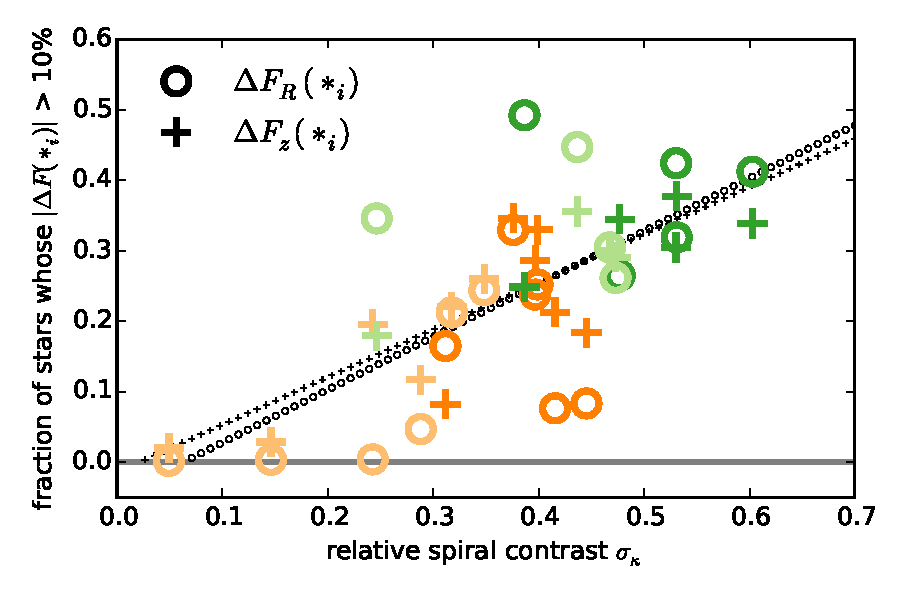
\includegraphics[width=\columnwidth]{fig/MNdHHdiffSph2_plot_stdkappa_vs_frac10star_2.pdf}
\caption{Influence of the spiral arm contrast within the survey volume on the recovery of the gravitational forces at the positions of the stars that entered the \RM{analysis}. The relative spiral contrast on the $x$-axis was quantified as $\sigma_\kappa \equiv \sigma[\kappa(r\leq r_\text{max})]$ according to Equation \eqref{eq:std_kappa} in Section \ref{sec:spiral_arm_kappa}. On the $y$-axis the fraction of stars is shown for which the radial (circle symbols) and vertical (cross symbols) force residual calculated from Equations \eqref{eq:delta_FR}-\eqref{eq:delta_Fz} is larger than 10\% (i.e., at $0$ all stars have good force measurements). The dotted lines (small circles and crosses) are linear fits to the radial and vertical force residual fraction, respectively, and are guides to the eye that show the clear and expected trend that in volumes with smaller spiral arm contrast, where comparably fewer stars are located in spiral arms, the axisymmetric best-fit model can recover the true gravitational forces also for more stars. \Wilma{[TO DO: Make sure all final analyses are in this plot.]}}
\label{fig:std_kappa_vs_frac10_stars}
\end{figure}
%====================

%====================
\begin{figure}[!htbp]
\centering
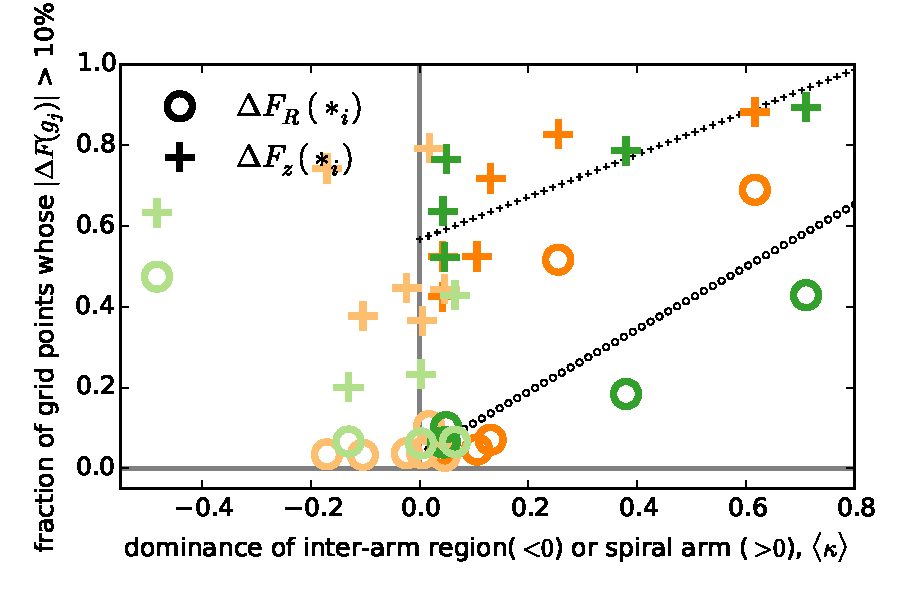
\includegraphics[width=\columnwidth]{fig/MNdHHdiffSph2_plot_meankappa_vs_frac10grid_2.pdf}
\caption{Influence of the spiral arm dominance within the survey volume on the "predictive power" of the models recovered from each survey volume. The spiral arm dominance on the $x$-axis was quantified as $\langle \kappa \rangle \equiv \langle \kappa(r\leq r_\text{max})\rangle$ from Equation \eqref{eq:mean_kappa} in Section \ref{sec:spiral_arm_kappa}. The $y$-axis shows the fraction of a large and fixed cylindrical volume with $r_\text{max}=5~\text{kpc}$ and $|z|1.5~\text{kpc}$ centred around the respective survey volume positions given in Table \ref{tbl:volume_positions} (i.e., fraction of regular grid points) with radial (circle symbols) and vertical (cross symbols) force residuals larger than 10\%.  This quantifies how well the model can predict the potential in a large portion of the galaxy and at $0$ the "predictive power" is best. The dotted lines (small circles and crosses) are guides to the eyes fitted to the analyses dominated by spiral arms at positions \texttt{S8} (dark orange) and \texttt{S5} (dark green) in Table \ref{tbl:volume_positions}. This figure demonstrates that the ''predictive power'' of a model derived from a survey volume that is either large enough for spiral arms not to dominate the volume ($\langle \kappa \rangle \sim 0$, compare Figure \ref{fig:spiral_arm_kappa}), or that are derived from volumes centered on inter-arm regions ($\langle \kappa \rangle \lesssim 0$, volumes at \texttt{I8}, bright orange, and \texttt{I5}, bright green) are less biased by the kinematics in the spiral arms and have therefore a higher predictive power. (The only exception is the volume at \texttt{I5} with $r_\text{max}=\Wilma{[TO DO]}$ and $\langle \kappa \rangle \sim -0.5$ that is especially strongly dominated by a depleted inter-arm region.)  \Wilma{[TO DO: Make sure all final analyses are in this plot.]} \Wilma{[TO DO: correct legend, it is supposed to read $\Delta F_R(g_j)$.]}}
\label{fig:mean_kappa_vs_frac10_grid}
\end{figure}
%====================


\subsubsection{Circular velocity curves and surface density profiles} \label{sec:circvel_surfdens}

In this section we will illustrate even further that even though the recovered potential parameters are very different for different survey volumes, the actual potential parameter recovery is very good---and not just the gravitational forces on average. In Appendix \ref{app:circsurf} in Figures \ref{fig:500pcSuite}-\ref{fig:5kpcSuite} we show the circular velocity curves and surface density profiles within two times the disk scale height ($|z|\leq 2 \times h_z = 0.34~\text{kpc}$) for all data sets in this work and compare them with the actual matter distribution in the angular wedge $\phi_0\pm \arcsin(r_\text{max}/R_0)$ containing the survey volume. We also mark the approximate radial regions in which the stellar number density per radial bin $\Delta R =200~\text{pc}$ is higher than average in each data set. Even though the curves vary extremely between the individual data sets, it becomes very obvious that it is indeed the regions in which the majority of stars is located that drives the \RM{} fit. And that, no matter if this region is dominated by a spiral arm or inter-arm region and no matter if this region is only as small as $r_\text{max}=500~\text{kpc}$, \RM{} is indeed constraining the local potential where most of the stars of the data set are located. Also, the constraints are not only most accurate but also most precise in these regions.

Only in the two volumes with $r_\text{max}=[0.5,1]~\text{kpc}$ at position \texttt{S8} \RM{} has some difficulties fitting the circular velocity curve; the model expects a flat or falling rotation curve and is presented with a steeply rising rotation curve due to the spiral arm dominating the region. But given \RM{} recovers a good average surface density profile and the circular velocity at least at the center of the small volume, the fit is still quite successful. 

In an application to real data in the MW we would also have the possibility to impose some informative prior information on the potential shape (e.g., on the rotation curve), to avoid very unrealistic results (see also discussion in Section \ref{sec:discussion_sun_location}).

\Jo{[TO DO: Jo writes: "It would be interesting to figure out a little more how we can determine whether we expect the fit to be strongly biased because we are using a volume that it sitting right on top of a massive spiral arm, although that is perhaps best kept for a later paper."]}

%-----------------------------------------------------------------------------------------------------------------------------------------------------------------------------
%DISCUSSION
%-----------------------------------------------------------------------------------------------------------------------------------------------------------------------------
\section{Discussion} \label{sec:discussion}

\subsection{On the informativeness of an orbit distribution function}

The qDF is surprisingly informative; even though there was absolutely no indication beforehand that the qDF would be actually a good model for the simulation snapshot; and even though small survey volumes dominated by non-axisymmetric spiral arms are definitely not well-described by the qDF. It appears however that a potential model that does not fit the gravitational forces acting on the stars must lead to such an unrealistic orbit/action distribution, that a fit with even such a simple orbit DF as the the qDF is impossible. This demonstrates once more how powerful the concept of an orbit DF is.

\subsection{On the restrictiveness of the parametrized potential model}

We do, on the one hand, use a bulge and halo model that reproduce the true bulge and halo better than we can hope to use one in reality for the MW. The fact that for all except of the largest volumes the true halo scale length is not remotely recovered (and some small volumes even have $f_\text{halo}=0$), and that the contribution of the bulge to the overall potential is small (i.e., the bulge contribution to the total radial force at $R=8~\text{kpc}$ is only $\sim 9-10\%$) remedies this apparent advantage. 

We use on the other hand a disk model, the Miyamoto-Nagai disk, that we chose purely for its convenient parametric form and of which we know that it is not a good model for the simulation snapshot, especially not for the radial density profile. As we saw in most figures in this work this might lead to biases in predicting the potential at radii where we have only a few or no stars. But because the spiral arms are such strong perturbations in the overall potential, a better disk model would not give much better results.

It appears that a potential model with a reasonable shape and flexibility (here: disk+bulge+halo structure with 5 free parameters) can do well enough in finding a good fit, both locally for small volumes and overall for large volumes.

\subsection{Precision of Gaia measurement errors}

Considering measurement uncertainties of distances and proper motions, we found in Paper I that for a survey volume with $r_\text{max} = 3~\text{kpc}$, distance uncertainties of <10\% and proper motion uncertainties of \Wilma{[TO DO]} \RM{} still gives unbiased parameter results. Even if the proper motion errors are not perfectly known. 

At a distance of $3~\text{kpc}$ the measurement uncertainties of bright stars in Gaia lie even below these limits. 

In paper I we focussed on recovering completely unbiased model parameters and found that \RM{} is robust to moderate deviations of the model assumptions. In this work we released the condition that the model parameters itself had to be recovered accurately, but allowed \RM{} to simply find an overall best fit for the data strongly affected by spiral arms---which was surprisingly successful in recovering the local potential even if the model parameters were not recovered. 

We therefore presume that in reality we probably have an even larger margin of error before the measurement uncertainties mess up the constraints noticeably than we found in Paper I. And Gaia uncertainties are already below our formal error.

In addition, we found in this work that a volume of $r_\text{max} = 3~\text{kpc}$ should be already big enough to find an overall best fit axisymmetric model for the galaxy. At larger distances dust starts affecting the measurements. And inside of $R=3-4~\text{kpc}$ the stellar motions become increasingly non-axisymmetric, possibly because  of the Galactic bar \citep{2014ApJ...783..130R}.

Overall we should therefore be very well off by applying \RM{} to Gaia data within $r_\text{max}=3~\text{kpc}$ only.

\subsection{Location of the Sun in the Milky Way} \label{sec:discussion_sun_location}

\Jo{[TO DO: Jo writes: "Perhaps section 5.4 could be quite a bit shorter, because it is quite speculative and seems oddly detailed given that it's speculative."]}

The Sun is located in one of the smaller spiral arms of the MW, the local Orion spur/arm \citep{1953ApJ...118..318M}. The Orion arm has long been considered a minor arm within the MW \citep{1985IAUS..106..335B}. Two of the MW's major spiral arms pass by the Sun within a few kpc: The Perseus arm is $\sim2~\text{kpc}$ from the Sun (towards the outer MW) \citep{2006Sci...311...54X}, and the Sagittarius arm at $\sim1~\text{kpc}$ \citep{2010PASJ...62..287S}. 

Although, recent observations of stronger star formation (SF) in the Orion arm \citep{2013ApJ...769...15X} and lower SF in the Perseus arm \citep{2013ApJ...775...79Z} suggest that the designation which arms in the MW are "major arms" could be slightly different than previously thought.

The Gaia DR1 in September 2016 will have parallax measurements better than 10\% within a maximum range of $\sim 500~\text{pc}$ from the Sun, the Gaia DR2 at the end of 2017 will cover $2~\text{kpc}$ with good parallaxes \HW{[TO DO: My only reference for this is HW. Some paper?]}.

How reliable \RM{} results from the DR1 will be, depends on the strength of the local Orion arm, which will dominate the survey volume. If previous assessments that it is only a weak spiral arm are correct, we can hope to get already pretty reliable measurements for the overall MW potential. If it is a stronger spiral arm, we might run into some difficulties when modelling such a small volume dominated by a spiral arm (see Figure \ref{fig:500pcSuite}).

However, a recent measurement of the MW's rotation curve by \citet{2014ApJ...783..130R} confirms again that it is flat. We could impose this condition as a prior constraint in \RM{} (or fix the rotation curve slope as \citet{2013ApJ...779..115B} did in their \RM{} analysis), which should greatly help \RM{} to find a good model even from a small volume on a strong spiral arm. 

In the Gaia DR2 with a coverage of $r_\text{max}\sim2~\text{kpc}$ we would in addition to the Orion arm also have the Sagittarius and Perseus arms cross the survey volume. \RM{} should do much better with this volume, because it should become easier to average over spiral arms and inter-arm regions if there are several of them.

The scatter and errors of the rotation curve measurements in Figure 4 by \citet{2014ApJ...783..130R} could hide spiral arm signatures as strong as those of the simulated spiral galaxy in this work. It is however more likely that the MW spiral arms are actually weaker than in this simulation: \citet{2014ApJ...783..130R} measured for example that typical peculiar non-circular motions in spiral arms were around $10~\text{km s}^{−1}$ (and around $20~\text{km s}^{−1}$ in the Perseus arm), while Figure \ref{fig:DF_velres} about the non-axisymmetric velocity distribution in our simulated galaxy suggests an excess of stars with radial velocities around $50~\text{km s}^{-1}$.

\citet{2014ApJ...783..130R} also found that within $R\sim 4~\text{kpc}$ the peculiar motions become much bigger, which could be due to the Galactic bar that stirs up the stellar motions in the center. For \RM{} a volume around the Sun of $r_\text{max}=3-4~\text{kpc}$ should however already give good results. 

\subsection{Recovering non-axisymmetric structures in the potential from modelling small volumes}

As we saw in Section \ref{sec:circvel_surfdens} and the Figures in Appendix \ref{app:circsurf}, \RM{} makes a very good attempt at fitting the local surface density and circular velocity curve also for volumes as small as $r_\text{max}=500~\text{pc}$ or $1\text{kpc}$. The modelling results might not always be informative about global properties of the potential (i.e., the recovered model does not have a halo, a too thick disk or a overall completely wrong rotation curve slope), but it does tell us about the local potential. It for example correctly predicts a higher surface density in survey volumes dominated by spiral arms, or correctly estimates the circular velocity curve at the median radial position of the stars. 

Instead of discarding these globally wrong potential models from small volumes we could actually make use of this interesting property of \RM{} modelling. First of all it implies that we can to a certain extent already trust modelling results from the Gaia DR1 with its small spatial coverage---in particular the gravitational forces at the solar position. At later stages, where we have the full Gaia catalogue with its huge survey volume, we could split the data set not only into different MAPs analogous to \citet{2013ApJ...779..115B}, but also into different spatial bins in the $(x,y)$ plane of the MW and model each of the smaller volumes separately. This approach would probe the local potential only, even when using an axisymmetric potential model, and should be sensitive to the spiral arms. In this way it should be possible to build up a non-axisymmetric map of the MW potential---with very large spatial pixels however---with constraints from dynamical modelling only. It would be in particular interesting to compare and correlate these results from action-based dynamical modelling with results from dynamical Jeans models of the MW disk, stellar number counts and gas disk measurements to also learn more about the non-axisymmetric distribution of dark matter in the MW disk.

%-----------------------------------------------------------------------------------------------------------------------------------------------------------------------------
%CONCLUSION
%-----------------------------------------------------------------------------------------------------------------------------------------------------------------------------
\section{Conclusion} \label{sec:conclusion}

\RM{} is a dynamical modelling machinery that simultaneously fits an action-based DF and axisymmetric potential model to the 6D phase-space coordinates of stellar populations in the MW disk and builds heavily on previous work by \citet{2011MNRAS.413.1889B,2012MNRAS.426.1324B,2015ApJS..216...29B}. In this work we have continued a throughout investigation of the capabilities of \RM{} to recover the MW's gravitational potential. \RM{} was first applied by \citet{2013ApJ...779..115B} and improved and tested in detail against the breakdowns of its modelling assumptions by \citet{2016arXiv160508601T}.  

Here, we investigated the important aspect of modelling data affected by spiral arms in the galactic disk with the axisymmetric \RM{} modelling. All similar studies using action-based modelling assume the influence of spiral arms not to be problematic, but here we test this assumption for the first time explicitly by modelling a simulated spiral galaxy by \citet{2013ApJ...766...34D} (which has stronger spiral arms as we expect in the MW) and by comparing the modelling results with the true potential. It turns out, that \RM{}-like action-based dynamical modelling is indeed very robust against perturbations of spiral arms, especially if the survey volume is large enough such that spiral-arms and inter-arm regions average out. In Section \ref{sec:results_part1} we demonstrated this in detail for a single \RM{} analysis of a data set with a spatial coverage of radius $r_\text{max}=4~\text{kpc}$ around the Sun.

We have investigated analyses in different survey volumes in the simulated galaxy in Section \ref{sec:results_part2}, with different sizes and at different positions with respect to the spiral arms and inter-arm regions. It turns out that independent of the size and position of the survey volume the gravitational forces are mostly well recovered at the locations of the stars that entered the analysis. Starting from survey volume sizes $r_\text{max}=3~\text{kpc}$ the recovered potential model becomes already a pretty good average potential model for the whole galaxy. For a convenient position, e.g., in a smooth and not too depleted inter-arm region, also smaller models can give good overall constraints. If a small volume is dominated by a very strong spiral arm the constraints become less reliable, as expected. The correct dark matter halo scale length was however only recovered for a survey volume as large as $r_\text{max}=5~\text{kpc}$. 

This overall robustness of \RM{} is in particular notable, as the breakdown of the assumption of axisymmetry implies a breakdown of several model assumptions simultaneously: (i) orbital actions are not conserved anymore, which dilutes the whole idea behind action-based DF modelling somewhat, (ii) the axisymmetric potential model is not expected to be an optimal model for the galaxy, (iii) the quasi-isothermal DF is used for its functional simplicity and was not expected to describe the orbit distribution within spiral arms. However, the qDF seems to be informative enough to guide the fit to potential shapes that correctly measure the average surface density within $\sim2 \times$ the disk scale height and the circular velocity where most of the stars that entered the analysis are located---even for small volumes with $r_\text{max}=500~\text{kpc}$ dominated by spiral arms.

All these results make us very optimistic that \RM{} will be well-suited to making new measurements of the MW's gravitational potential with the upcoming Gaia releases. It might work potentially even with the Gaia DR1, that only covers a small region $r_\text{max}=500~\text{kpc}$ (where the distance errors are small enough), because the local Orion arm, in which the Sun lies, is thought to be only a minor spiral arm in the MW and should not disturb the modelling too much. 


%-----------------------------------------------------------------------------------------------------------------------------------------------------------------------------
%APPENDIX
%-----------------------------------------------------------------------------------------------------------------------------------------------------------------------------

\bibliography{references_paper2}{}
\bibliographystyle{aasjournal}

\begin{appendix}

\section{Circular velocity curves and surface density profiles for different survey volumes} \label{app:circsurf}

\Jo{[TO DO: Jo writes: "I'm also not sure that the appendix is really necessary, although there are few disadvantages to keeping it."]}

This appendix presents in Figures \ref{fig:500pcSuite}-\ref{fig:5kpcSuite} all circular velocity curves and surface density profiles that were recovered in this work from survey volumes of different sizes $r_\text{max} \in [0.5,1,2,3,4,5]~\text{kpc}$ and positions (see Table \ref{tbl:volume_positions}). The surface density profiles are calculated within twice the disk scale height $|z| \leq 2\times h_z=0.34~\text{kpc})$, because this encloses most of the mass in the disk, most tracers and is therefore a height that should be well constrained by \RM{}. \Wilma{[TO DO: Redo plots A3-A6 with a fixed radial bin size for the histograms.]}

%====================
\begin{figure*}[!htbp]
\centering
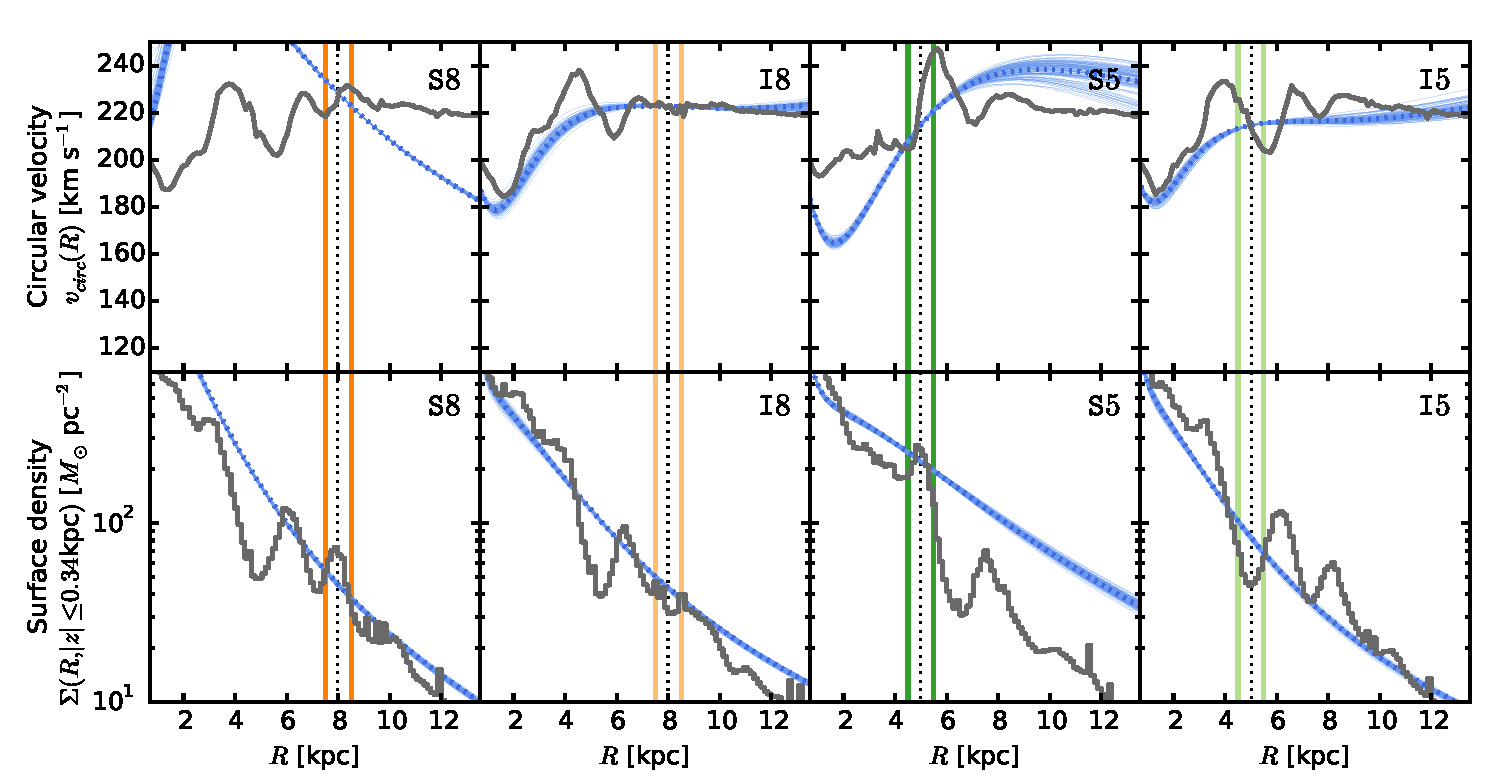
\includegraphics[width=0.8\textwidth]{fig/MNdHHdiffSph2_vcirc_surfdens_500pcSuite.pdf}
\caption{Comparison of the true local circular velocity curve and surface density within$|z| \leq 2 \times h_z = 0.34~\text{kpc}$ with the recovered \RM{} models from survey volumes of size $r_\text{max}=500~\text{pc}$. The grey curves show the profiles as derived from the galaxy simulation snapshot and averaged over an angular wedge $\phi_0\pm\arcsin(r_\text{max}/R_0)$ that encloses the corresponding survey volume (see Table \ref{tbl:volume_positions} for the corresponding $R_0$ and $\phi_0$ values, i.e., that part of the spiral galaxy that was probed by the data. The vertical orange and green lines mark the radial extent of the survey volume and the dotted vertical line marks the mean radius of all stars that entered the analysis. The blue lines finally show the \RM{} potential models recovered from these stars; the blue dotted line corresponds to the model with the median potential parameters, and the thin blue lines correspond to 100 potential models drawn from the full posterior probability distribution sampled with the MCMC. It turns out that the constraints of highest accuracy and precision are always where most of the stars are located---within the survey volume and in particular at the peak of the distribution. \Wilma{[TO DO: Make sure all final analyses are in this plot.]} \Wilma{[TO DO: \RM{} analysis of the data set centered on \texttt{I5} is still running.]}}
\label{fig:500pcSuite}
\end{figure*}
%====================

%====================
\begin{figure*}[!htbp]
\centering
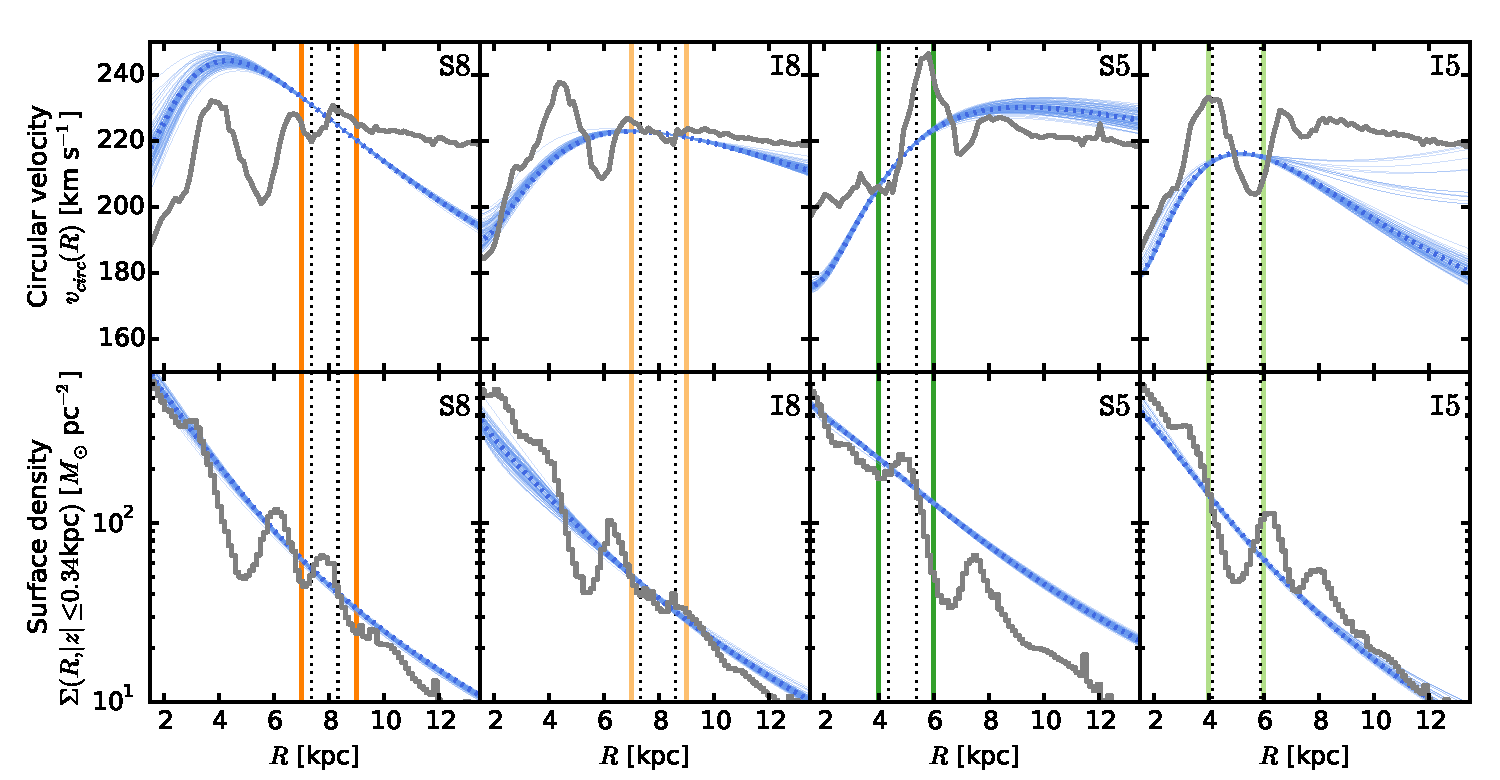
\includegraphics[width=0.8\textwidth]{fig/MNdHHdiffSph2_vcirc_surfdens_1kpcSuite.pdf}
\caption{Same as Figure \ref{fig:500pcSuite}, but for all survey volumes with $r_\text{max}=1~\text{kpc}$. \Wilma{[TO DO: Make sure all final analyses are in this plot.]}}
\label{fig:1kpcSuite}
\end{figure*}
%====================

%====================
\begin{figure*}[!htbp]
\centering
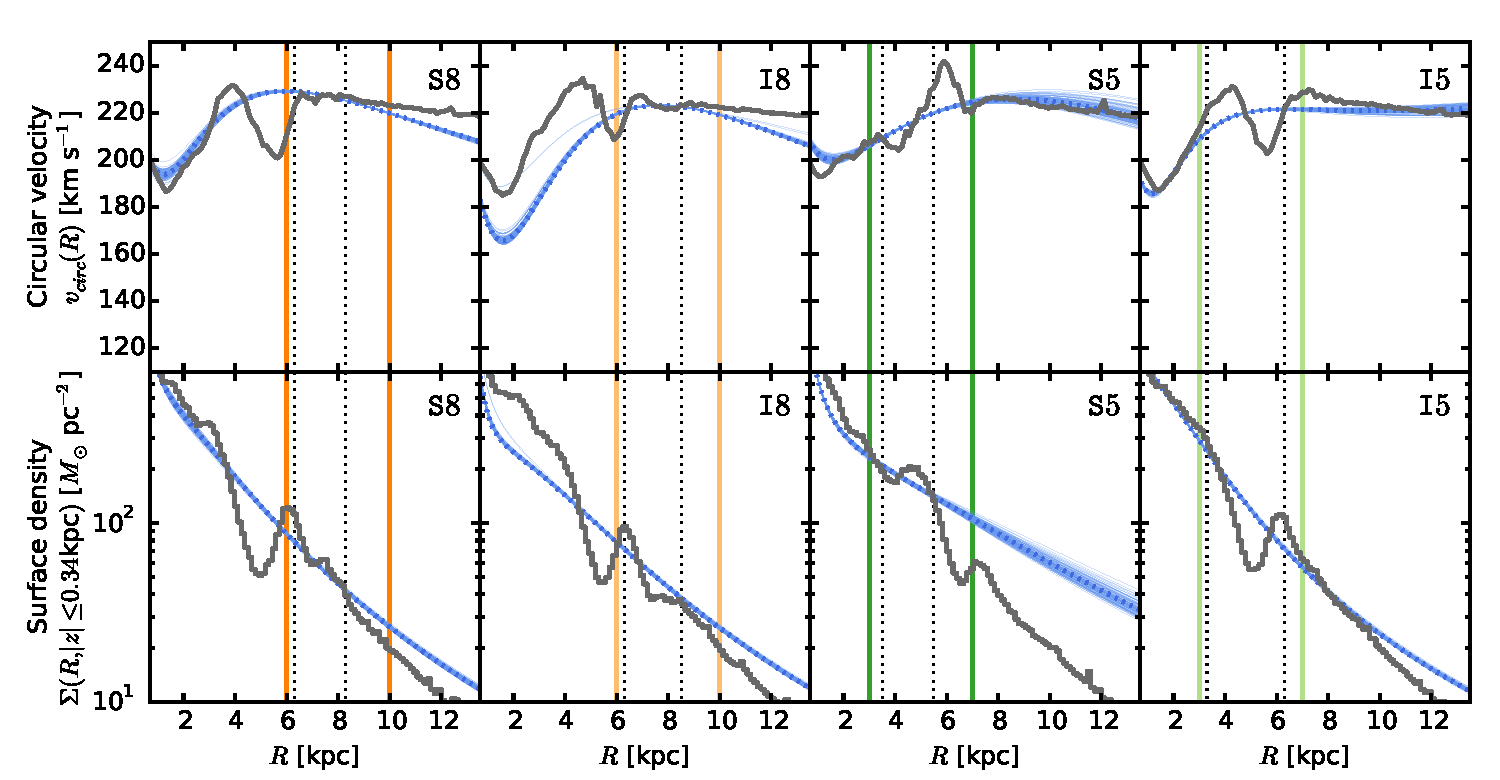
\includegraphics[width=0.8\textwidth]{fig/MNdHHdiffSph2_vcirc_surfdens_2kpcSuite.pdf}
\caption{Same as Figure \ref{fig:500pcSuite}, but for all survey volumes with $r_\text{max}=2~\text{kpc}$. Instead of marking the median of the radial stellar distribution, the dotted lines correspond here to the radial range within which the number of stars per radial bin $\Delta R = 200~\text{pc}$ is higher than average. This appears to be also the range within which the constraints are best. \Wilma{[TO DO: Make sure all final analyses are in this plot.]}}
\label{fig:2kpcSuite}
\end{figure*}
%====================

%====================
\begin{figure*}[!htbp]
\centering
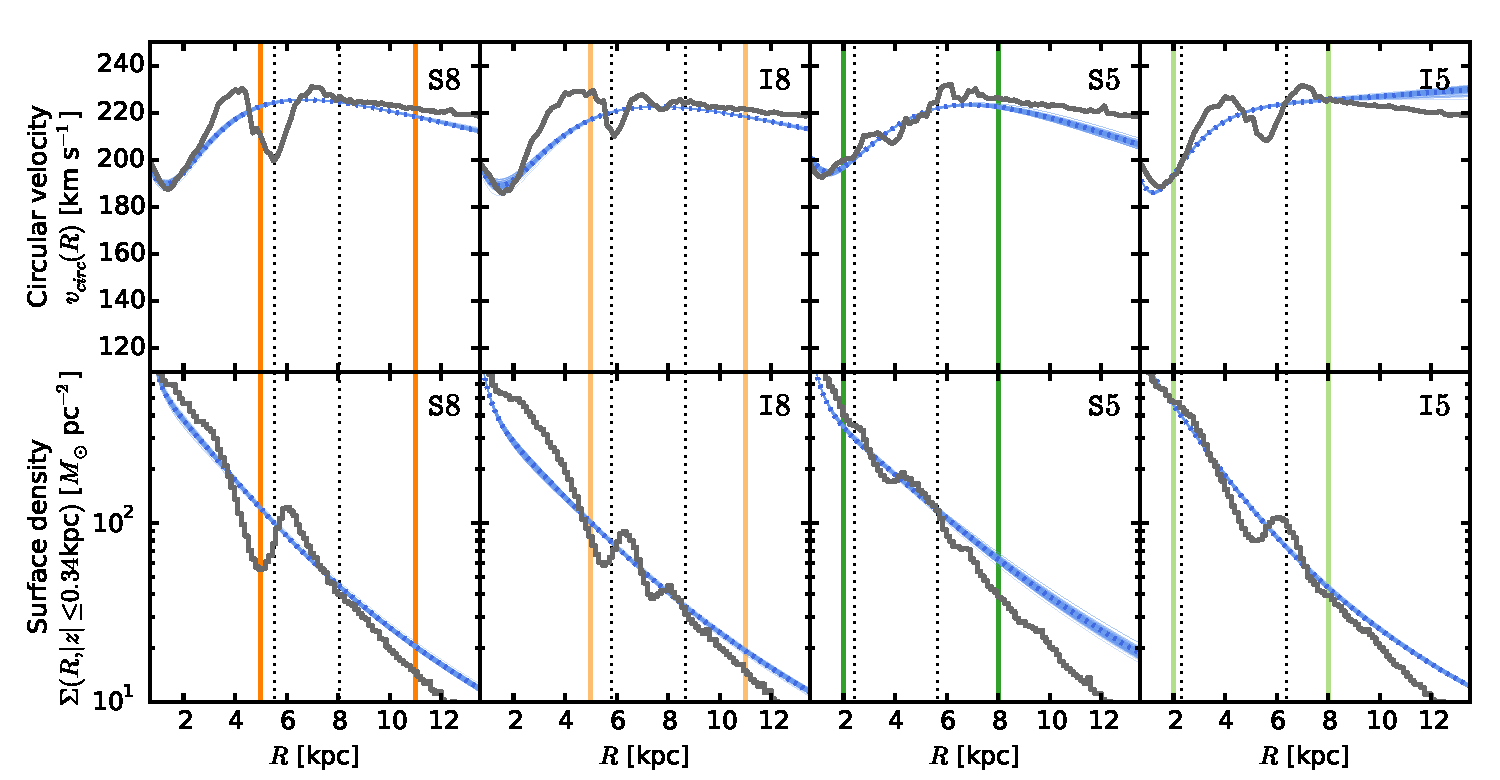
\includegraphics[width=0.8\textwidth]{fig/MNdHHdiffSph2_vcirc_surfdens_3kpcSuite.pdf}
\caption{Same as Figure \ref{fig:2kpcSuite}, but for all survey volumes with $r_\text{max}=3~\text{kpc}$. \Wilma{[TO DO: Make sure all final analyses are in this plot.]}}
\label{fig:????}
\end{figure*}
%====================

%====================
\begin{figure*}[!htbp]
\centering
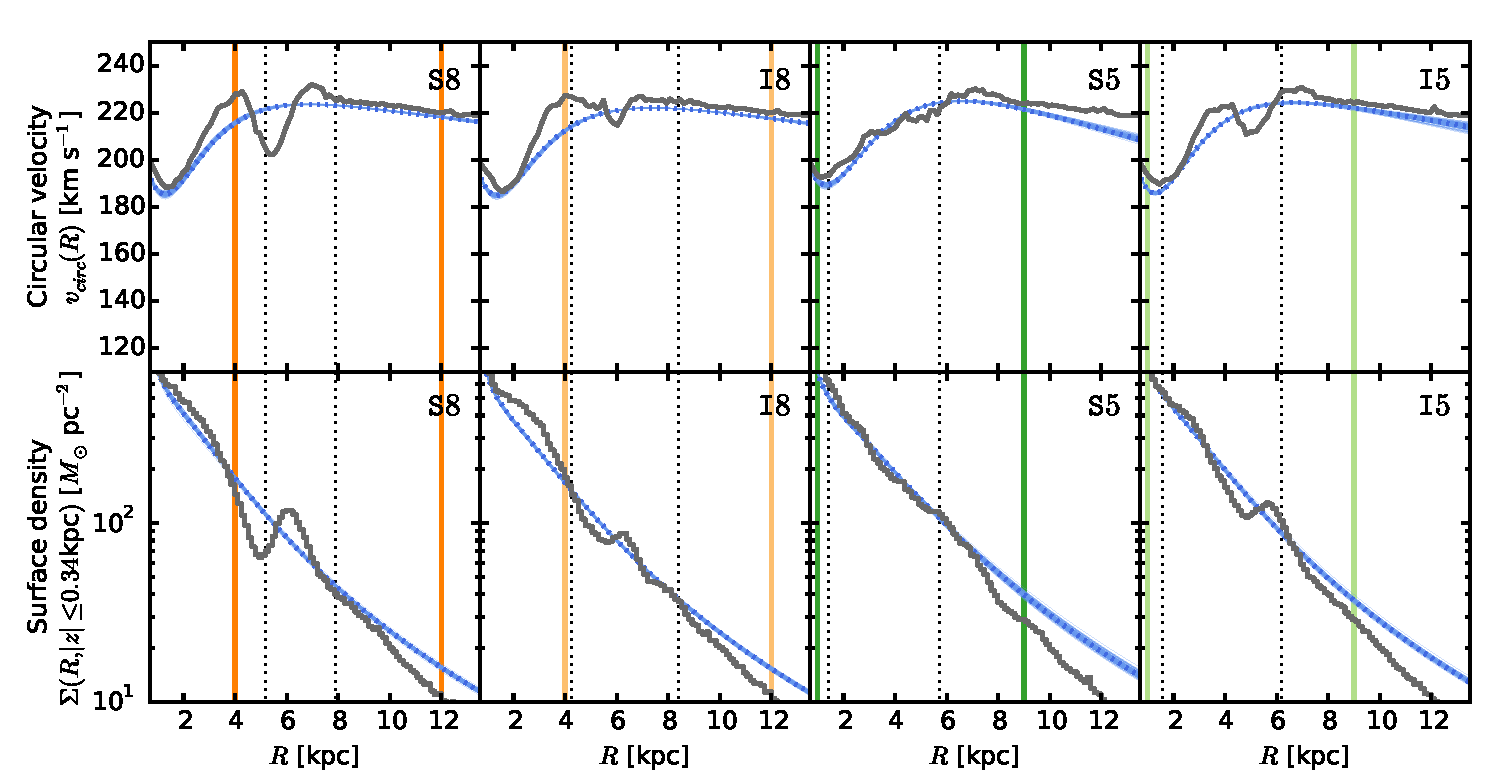
\includegraphics[width=0.8\textwidth]{fig/MNdHHdiffSph2_vcirc_surfdens_4kpcSuite.pdf}
\caption{Same as Figure \ref{fig:2kpcSuite}, but for all survey volumes with $r_\text{max}=4~\text{kpc}$. \Wilma{[TO DO: Make sure all final analyses are in this plot.]}}
\label{fig:????}
\end{figure*}
%====================

%====================
\begin{figure*}[!htbp]
\centering
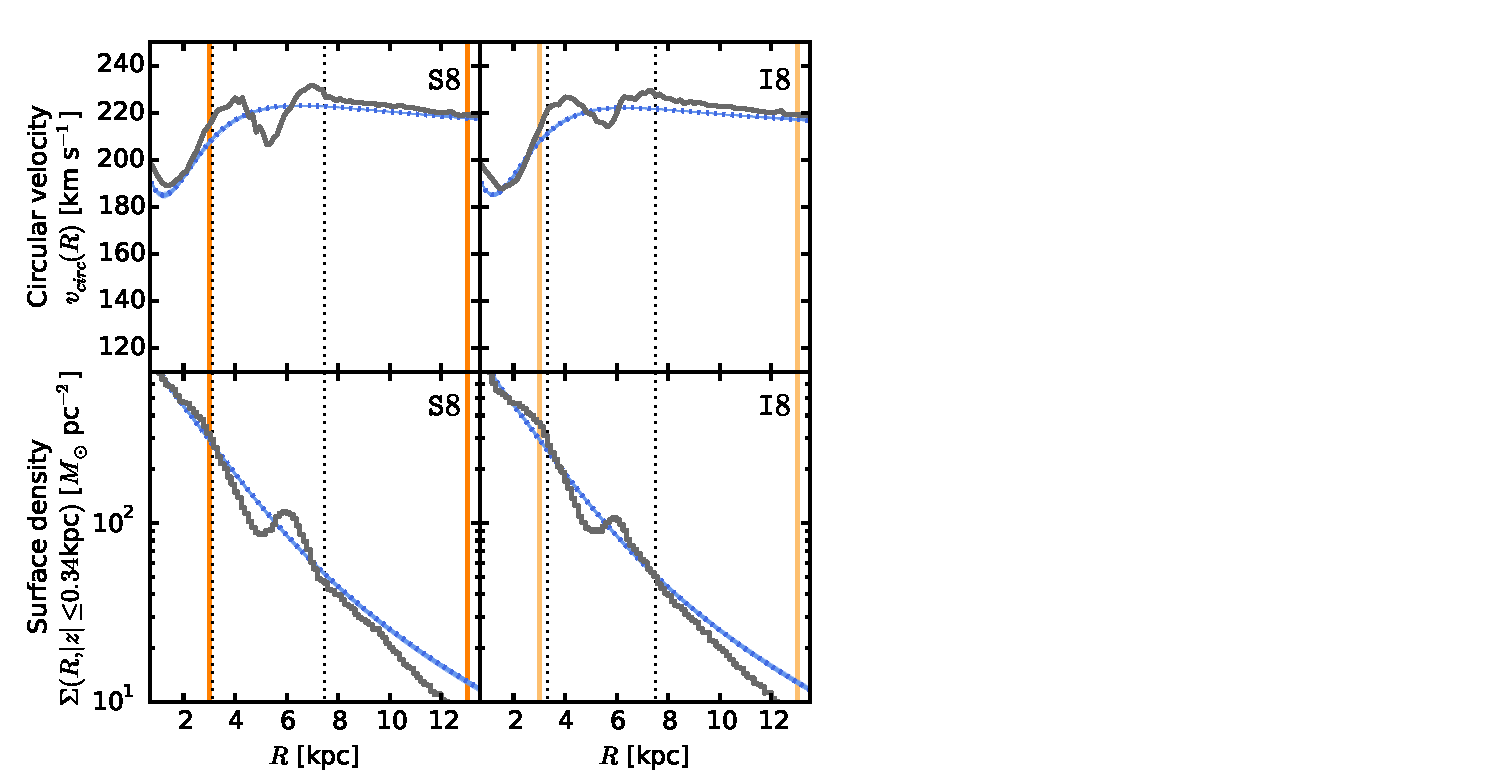
\includegraphics[width=0.8\textwidth]{fig/MNdHHdiffSph2_vcirc_surfdens_5kpcSuite.pdf}
\caption{Same as Figure \ref{fig:2kpcSuite}, but for all survey volumes with $r_\text{max}=5~\text{kpc}$. \Wilma{[TO DO: Make sure all final analyses are in this plot.]}}
\label{fig:5kpcSuite}
\end{figure*}
%====================

\end{appendix}

\end{document}